\documentclass[12pt]{article}
\usepackage[english]{babel}
\usepackage{url}
\usepackage[utf8]{inputenc}
\usepackage{rotating}
\usepackage{listings}
\usepackage[
backend=biber,
style=numeric,
urldate=long
]{biblatex}
\usepackage{booktabs}
\newcommand{\tabitem}{\makebox[1em][r]{\textbullet~}}
\usepackage{amsmath}
\usepackage{graphicx}
\usepackage[toc,page]{appendix}
\graphicspath{{images/}}
\usepackage{setspace}
\usepackage{parskip}
\usepackage{fancyhdr}
\usepackage{vmargin}
\usepackage{float}
\usepackage{chngcntr}
\usepackage [autostyle, english = british]{csquotes}
\MakeOuterQuote{"}
\usepackage[format=plain,
            labelfont={bf,it},
            textfont=it,
            justification=centering]{caption}
\usepackage{subcaption}
\counterwithin{figure}{section}
\counterwithin{table}{section}
\setmarginsrb{3 cm}{2.5 cm}{3 cm}{2.5 cm}{1 cm}{1.5 cm}{1 cm}{1.5 cm}

\usepackage{xcolor}

\colorlet{punct}{red!60!black}
\definecolor{background}{HTML}{EEEEEE}
\definecolor{delim}{RGB}{20,105,176}
\colorlet{numb}{magenta!60!black}

\usepackage[T1]{fontenc}
\usepackage{inconsolata}

\usepackage{color}

\definecolor{pblue}{rgb}{0.13,0.13,1}
\definecolor{pgreen}{rgb}{0,0.5,0}
\definecolor{pred}{rgb}{0.9,0,0}
\definecolor{pgrey}{rgb}{0.46,0.45,0.48}

\lstdefinelanguage{json}{
    basicstyle=\normalfont\ttfamily,
    numbers=left,
    numberstyle=\scriptsize,
    stepnumber=1,
    numbersep=8pt,
    showstringspaces=false,
    breaklines=true,
    frame=lines,
    backgroundcolor=\color{background},
    literate=
     *{0}{{{\color{numb}0}}}{1}
      {1}{{{\color{numb}1}}}{1}
      {2}{{{\color{numb}2}}}{1}
      {3}{{{\color{numb}3}}}{1}
      {4}{{{\color{numb}4}}}{1}
      {5}{{{\color{numb}5}}}{1}
      {6}{{{\color{numb}6}}}{1}
      {7}{{{\color{numb}7}}}{1}
      {8}{{{\color{numb}8}}}{1}
      {9}{{{\color{numb}9}}}{1}
      {:}{{{\color{punct}{:}}}}{1}
      {,}{{{\color{punct}{,}}}}{1}
      {\{}{{{\color{delim}{\{}}}}{1}
      {\}}{{{\color{delim}{\}}}}}{1}
      {[}{{{\color{delim}{[}}}}{1}
      {]}{{{\color{delim}{]}}}}{1}
}

\lstdefinestyle{MyJava}{language=Java,
    basicstyle=\normalfont\ttfamily,
    numbers=left,
    numberstyle=\scriptsize,
    stepnumber=1,
    numbersep=8pt,
    breaklines=true,
    postbreak=\raisebox{0ex}[0ex][0ex]{\ensuremath{\color{red}\hookrightarrow\space}},
    frame=lines,
    backgroundcolor=\color{background},
  showspaces=false,
  showtabs=false,
  showstringspaces=false,
  breakatwhitespace=true,
  commentstyle=\color{pgreen},
  keywordstyle=\color{pblue},
  stringstyle=\color{pred},
  moredelim=[il][\textcolor{pgrey}]{$$},
  moredelim=[is][\textcolor{pgrey}]{\%\%}{\%\%}
}

\usepackage{etoolbox}
\patchcmd{\theindex}{\thispagestyle{fancy}}{}{}{}

\title{NewSumm}								% Title
\author{Kunal M L Wagle}								% Author
\date{\today}											% Date


\addbibresource{sample.bib}

\DefineBibliographyStrings{english}{%
urlseen = {Retrieved},
}

\makeatletter
\let\thetitle\@title
\let\theauthor\@author
\let\thedate\@date
\makeatother

\usepackage{imakeidx}
\indexsetup{othercode=\small}
\makeindex[program=makeindex,columns=2,intoc=true,options={-s mystyle.ist}]

\pagestyle{fancy}
\fancyhf{}
\rhead{\theauthor}
\lhead{\thetitle}
\cfoot{\thepage}

\begin{document}

%%%%%%%%%%%%%%%%%%%%%%%%%%%%%%%%%%%%%%%%%%%%%%%%%%%%%%%%%%%%%%%%%%%%%%%%%%%%%%%%%%%%%%%%%

\begin{titlepage}
	\centering
    \vspace*{0.5 cm}
    
\includegraphics[scale = 0.05]{Imperial_College_London_crest.png}\\[1.0 cm]	% University Logo
    \textsc{\LARGE Imperial College London}\\[2.0 cm]	% University Name
	\textsc{\Large C401}\\[0.5 cm]				% Course Code
	\textsc{\large MEng Computing Final Report}\\[0.5 cm]				% Course Name
	\rule{\linewidth}{0.2 mm} \\[0.4 cm]
	{ \huge \bfseries \thetitle \\[0.4cm] \textsc{\large News Aggregator and Summariser}}\\
	\rule{\linewidth}{0.2 mm} \\[1.5 cm]
	
	\begin{minipage}{0.4\textwidth}
		\begin{flushleft} \large
			\emph{Author:}\\
			\theauthor
			\end{flushleft}
			\end{minipage}~
			\begin{minipage}{0.4\textwidth}
			\begin{flushright} \large
			\emph{Supervisor:} \\
			Anandha Gopalan									% Your Student Number
		\end{flushright}
	\end{minipage}\\[2 cm]
	
	{\large \thedate}\\[2 cm]
 
	\vfill
	
\end{titlepage}

%%%%%%%%%%%%%%%%%%%%%%%%%%%%%%%%%%%%%%%%%%%%%%%%%%%%%%%%%%%%%%%%%%%%%%%%%%%%%%%%%%%%%%%%%

\section*{Abstract}
Abstract to be written

\pagebreak

\section*{Acknowledgements}

Acknowledgements to be written

\clearpage

\doublespacing
\tableofcontents
\pagebreak
\listoffigures
\pagebreak
\listoftables
\pagebreak
\lstlistoflistings
\singlespacing
\pagebreak

%%%%%%%%%%%%%%%%%%%%%%%%%%%%%%%%%%%%%%%%%%%%%%%%%%%%%%%%%%%%%%%%%%%%%%%%%%%%%%%%%%%%%%%%%


\section{Introduction}

\subsection{The Problem}

\subsubsection{The Media}

The Fourth Estate is currently enduring one of its toughest passages of time to date. Some of the challenges it faces are familiar, whilst some are new ones that have been created by the onset of the digital age. 

The term "fake news" is now at the forefront of our minds in an atmosphere that is highly charged. The Digital News Report 2016 found that in the United Kingdom only 50\% of readers trust what they say in the news, whilst only 29\% say that they trust journalists (see Figure \ref{TrustInNews}). This statistics appear to be even more dire for the media in the Untied States of America, when the percentages are 33\% for news channels, and 27\% for print journalists.

\begin{figure}[h]
  \centering
    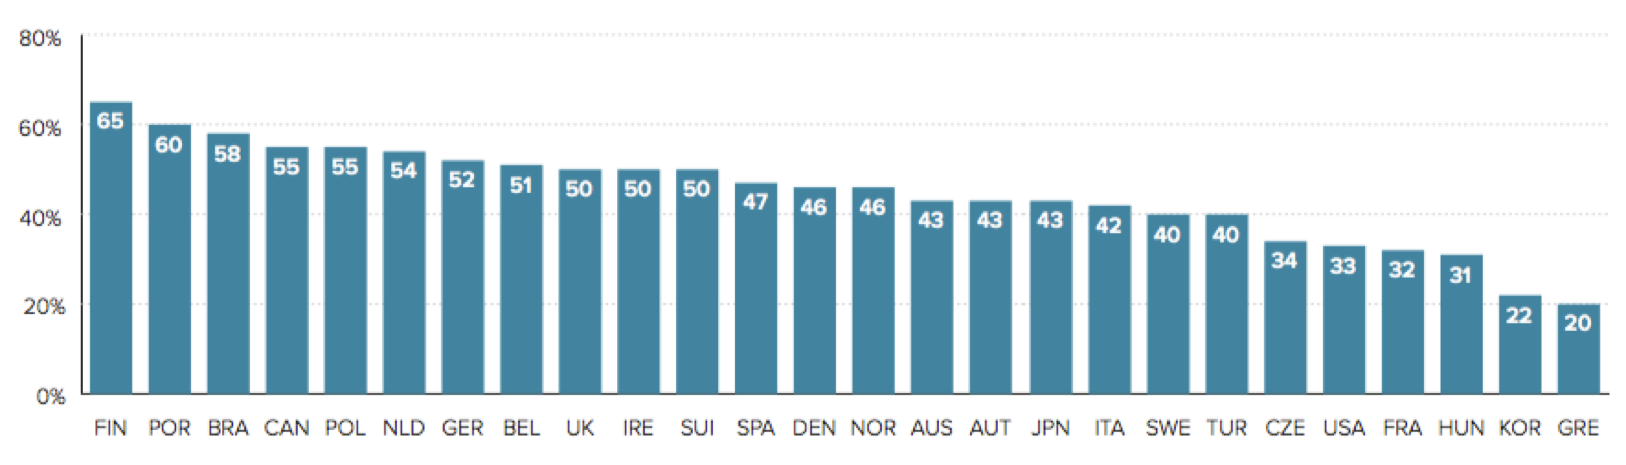
\includegraphics[width=\textwidth]{TrustInNews.png}
   \caption[The Digital News Report 2016 on trust in the news]{Digital News Report findings showed that when it came to trust in the news, in only a few countries was trust as high as 50\% in the accuracy of a piece of news. In countries such as the United States it is far lower.}
   \label{TrustInNews}
\end{figure}

In addition to this, the media have been submerged in a deluge of websites that also claim to disseminate news to readers. In an increasingly digital world, anyone with access to the internet could write a blog about a news story. The popularity of social networks such as Facebook and Twitter also mean that these amateur "journalists" have a platform on which they can compete with professionals from the industry. 

In 2016, the concept of fake news dominated the general election in the United States. Shortly after the country went to the polls, Hillary Clinton's campaign became dogged in rumour after more than a million tweets were sent out about the "pizzagate" scandal. The fake news went both ways. In July 2016, it was reported widely on blogs that Donald Trump had said in an interview with \emph{People} in 1998 that: 

\begin{displayquote}\emph{
"If I were to run, I'd run as a Republican. They're the dumbest group of voters in the country. They believe anything on Fox News. I could lie and they'd still eat it up. I bet my numbers would be terrific."}

\end{displayquote}

The claim was later found to have been fabricated.

Fake news and the people's trust is not the only major issue facing the media at the moment. Another key is sheer volume. Given the abundance of media outlets in the world at the moment, and perhaps more importantly (due to the internet) the accessibility around the globe, there is a lot of competition between outlets. 

\subsubsection{The Consumer}

As a result of a lot of the aforementioned accessibility, consumers also have a challenge in that they can't efficiently read all the news that is out there. If I were to search Google News on the 24th May 2017 for news about Donald Trump, I'd find a story about the President's meeting with the Pope at the Vatican (see Figure \ref{DonaldTrumpPope}). On further inspection, I can see that there are several pages of results about the meeting itself, from dozens of different news sources. A consumer has little to no hope of reading all of these.

\begin{figure}[h]
  \centering
    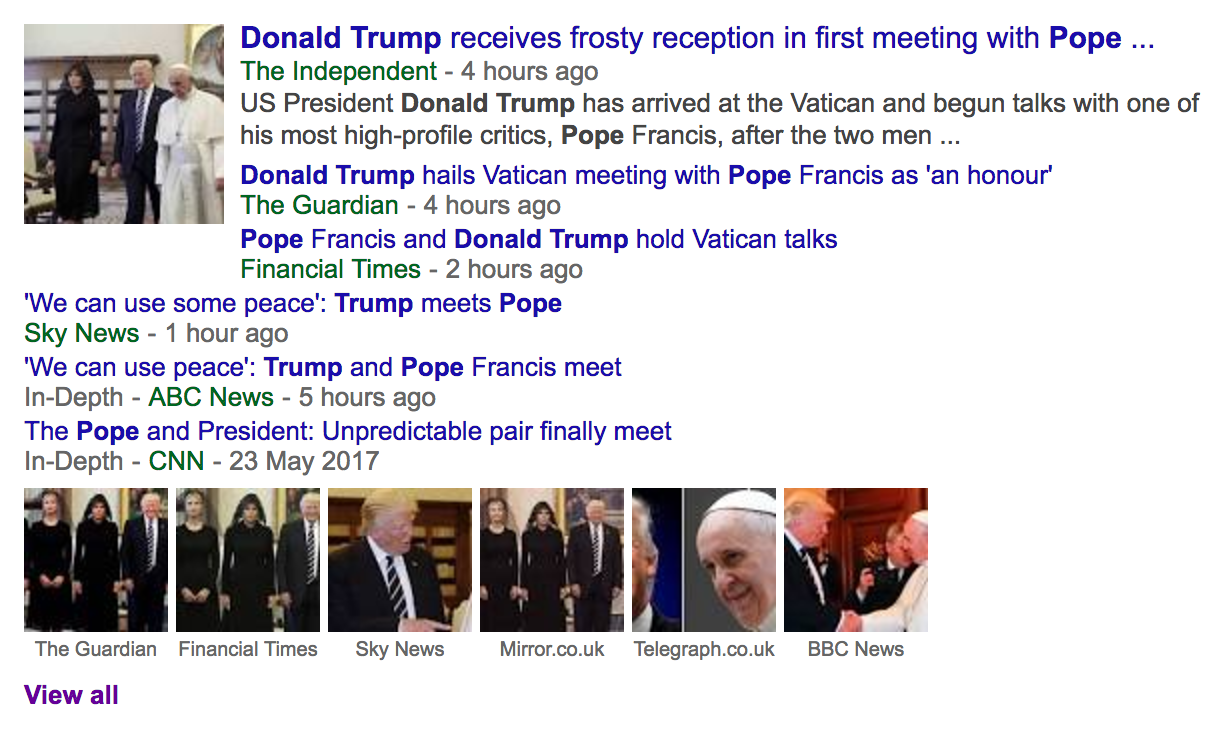
\includegraphics[scale=0.6]{DonaldTrumpPope.png}
   \caption[A Google News Search on 24th May 2017]{A Google News search for stories about President Trump's visit to the Vatican on 24th May 2017}
   \label{DonaldTrumpPope}
\end{figure}

So which news sources should a consumer prioritise? Often, that comes down to political opinion. In fact, the Digital News Report 2016, conducted by the Reuters Institute for the Study of Journalism, says that only 34\% of consumers in the United Kingdom believe that the media is "free from undue political influence". In the United States, which doesn't have a state broadcaster like the United Kingdom does in the BBC, the corresponding statistic is significantly lower at 21\%.

The immediate consequence of statistics like this is that if someone hasn't read all the sources in a piece of news, they are reasonably likely to develop some form of political bias on the issue (perhaps without even realising it). For example, someone who reads about a story in a left-leaning publication such as \emph{The Guardian} may feel differently when compared to someone who reads the corresponding story in a right-leaning publication such as \emph{The Daily Mail}. 

The simple solution to this would be reading the story in as many sources as possible before forming a final opinion. However, as mentioned before, this is just simply not feasible. In July 2016 a study was conducted by the Statistic Brain Research Institute that said that the average attention span of a person is now as low as 8.25 seconds. In addition to this, the Institute's findings also said that the average person only reads 28\% of a webpage of average length (593 words). Another key finding was that users spend only 4.4 seconds to cover each additional 100 words on a webpage. It's simply not possible for every news source to capture a user's attention, especially if they are all broadly covering the same story.

\subsection{News Aggregator and Summariser: A potential solution}

The fundamental aim of my project would be to create a project that directly addresses the consumer's concerns mentioned above, whilst indirectly aiding the concerns of the media.

The project would be a News Aggregator, that would allow users to see the news from multiple mainstream (and therefore "trusted") sources in one place. In addition to this though, the aggregator would also act as a summariser, so that a user doesn't need to read as much as before to gain the same opinion.

However, a key aim has to be to address the issue of there just simply being too much news for someone (who is reading from multiple sources) to take in. To try and achieve this, the News Aggregator will need to identify articles across sources that are about the same topic (for example, Donald Trump's visit to the Vatican), and summarise them. This will mean that a user only has to read a single article to get the full information from multiple sources about a news piece.

In an indirect attempt to allay the concerns of the media and the public about the phenomena that is fake news the News Aggregator will need to find a way to counteract it. One obvious way to do this would be through the limitation of the number of outlets to only those that are "trusted". In addition to this, a clear indication when reading the summary of what facts different outlets all agree on, and what facts they either differ on or omit, will allow the user to easily corroborate parts of the story.

A further secondary aim to this could be to allow a user to customise their summary, taking in information from the outlets of their choice (from the original "trusted" list). The advantage to this would potentially be that if a user decides that too many issues from one source are uncorroborated, they can remove them, and see only information from the other sources that have written about a topic. The disadvantage to this could be that if a user dismisses an entire section of the political spectrum as fake continuously, they'll still pick up a political bias on the facts of the topic. Although, it could be said that the Digital News Report 2016 findings suggest that this is a feature that won't be used much. One of the more interesting findings in the report was that more than 60\% (in the United Kingdom) were concerned about the potential impact of personalising their news feeds. They felt that it could lead to both "missing information" and "missing challenging viewpoints". 

%%%%%%%%%%%%%%%%%%%%%%%%%%%%%%%%%%%%%%%%%%%%%%%%%%%%%%%%%%%%%%%%%%%%%%%%%%%%%%%%%%%%%%%%%

\pagebreak

\section{Market Research}

\subsection{News Reading Habits}

\subsubsection{Digital News Report 2016}

\label{DigitalNewsReport}

Conducted by the Reuters Institute for the Study of Journalism\cite{reutersInstitute}\index{Reuters Institute for the Study of Journalism} in Oxford University\cite{oxford}\index{University of Oxford}, the Digital News Report\index{Digital News Report}\cite{digitalNewsReport} is an annual study that serves to investigate how people access and find out about news in various countries across the globe, including the United Kingdom\index{United Kingdom}.

The study attempts to cover, amongst other things how people get the news, how they use social media\index{Social Media}, what types of news they trust, and both the reasons to use and concerns about news aggregators. Findings of the report relevant to my concept are listed below:

\textbf{Reasons to use News Aggregators\index{News Aggregator!Reasons for use}}

\begin{figure}[h]
  \centering
    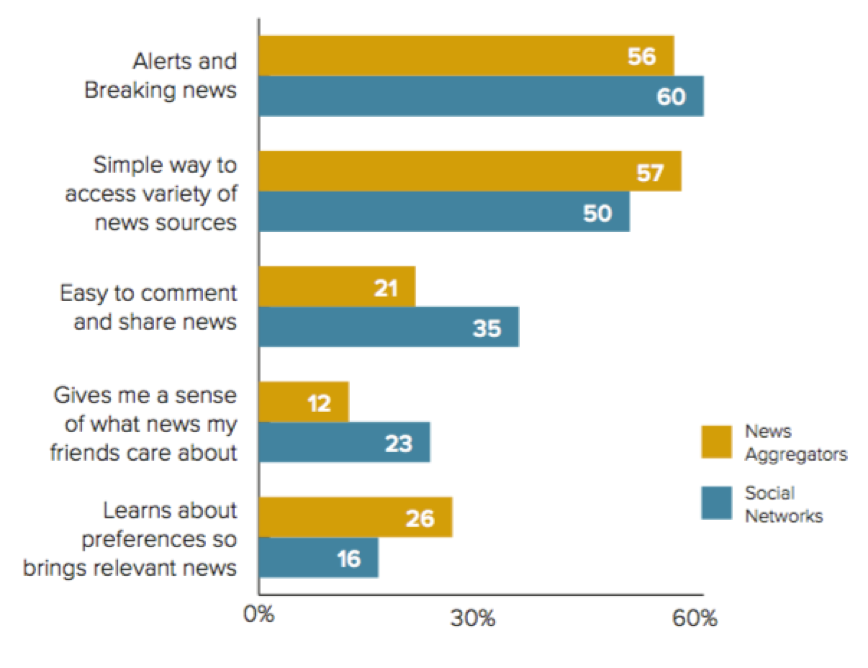
\includegraphics[scale=0.6]{WhySocialAggregatedNews.png}
   \caption[Why people use News Aggregators]{A graph showing why people use News Aggregators and Social Networks as news sources}
   \label{WhySocialAggregatedNews}
\end{figure}

As shown in the graph in Figure \ref{WhySocialAggregatedNews} the key to the popularity of a News Aggregator is that it's simplicity and speed. It's important to bring news as soon as it happens, and it needs to provide access to a variety of different news sources. Of lesser importance is the social aspect - the need to comment and share the news, although the fact that 26\% of people want their preferences to influence the news that they're interested in should not be discounted.

\textbf{Concerns about Personalised News\index{News ! Personalised}}

\begin{figure}[h]
  \centering
    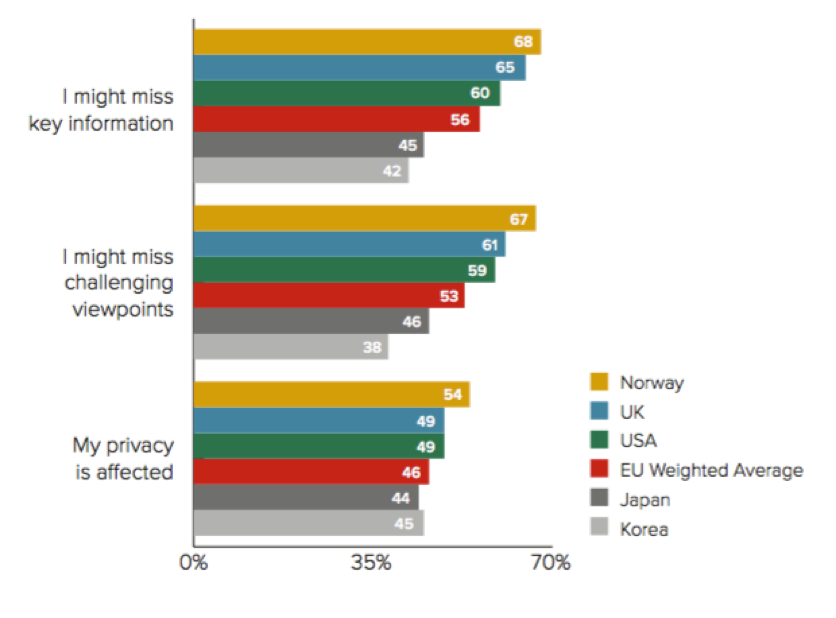
\includegraphics[scale=0.6]{PersonalisedNewsConcerns.png}
   \caption[Concerns with personalisation of News Feeds]{A graph showing the main three concerns that people have with Personalised News Feeds determining what they read.}
   \label{PersonalisedNewsConcerns}
\end{figure}

Key concerns, especially in the United Kingdom\index{United Kingdom}, with Personalised News\index{News ! Personalised} is that information might be incomplete. It is not difficult to see why this may be a concern - if you limit your news to a subset of the sources that might be available then it's possible to miss parts of the story - the parts that challenge aspects of the articles you're reading. It's therefore important that the project reflects this concern, which is why it is listed as a secondary aim (See section \ref{ChallengingViewpoints}). \\

\textbf{What should determine what someone reads next}

\begin{figure}[h]
  \centering
    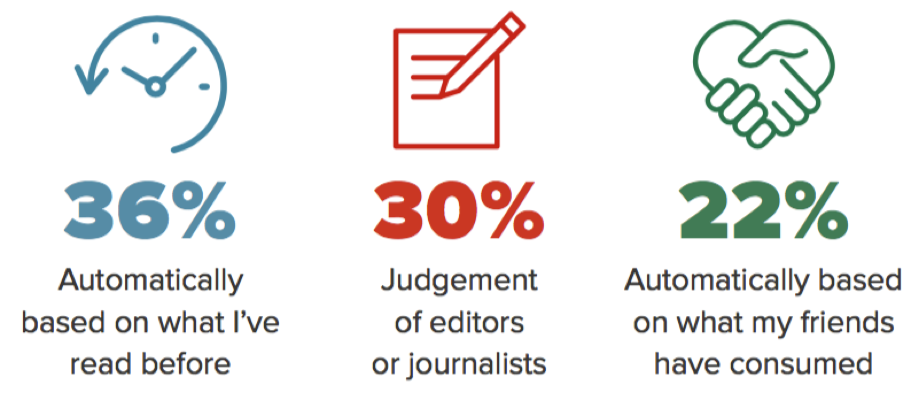
\includegraphics[scale=0.6]{HowPeopleTrustNews.png}
   \caption[What is a good way to get to the news?]{Key statistics in response to the question: Is this a good way to get the news?}
   \label{HowPeopleTrustNews}
\end{figure}

Least popular are algorithms that present news based on what people's friends have been reading. In general, according to the Reuters Institute\cite{reutersInstitute}\index{Reuters Institute for the Study of Journalism}, "People think *they* are the best judge of what's important to them." More interesting, is that people are now less inclined to allow journalists or editors to push articles to the top of reading lists than having an algorithm suggest similar stories to what they've just consumed. This could perhaps indicate that they aren't as trusting in journalists and editors as before - something that the Reuters Institute\index{Reuters Institute for the Study of Journalism} touches upon in an essay near the end of the report. \\

\textbf{Conclusions}

The Reuters Institute for the Study of Journalism\index{Reuters Institute for the Study of Journalism} is a trusted and respected organisation, and this study has been supported by institutions varying from media outlets such as the BBC\cite{bbc}\index{BBC}, news search engines such as Google\index{Google}\index{Google!Search Engine}, and other Universities, such as University of Canberra\cite{canberra}\index{University of Canberra}. Importantly, it's also supported by regulators, including Ofcom\cite{ofcom}\index{Ofcom}, which is the regulator in the United Kingdom\index{United Kingdom}. 

The survey was conducted on their behalf by YouGov\cite{yougov}\index{YouGov}, which is a highly respected polling company in the United Kingdom\index{United Kingdom}, and it surveyed more than 50,000 people, including over 2000 in the United Kingdom. In addition, the report is coupled with numerous essays on various key points that arose from the study. The writers of these essays varied from the Director of Research at the Reuters Institute\index{Reuters Institute for the Study of Journalism} to the Chief Executive Officer of The New York Times\cite{newYorkTimes}\index{New York Times}.

As a result of this, I deemed the Digital News Report 2016\index{Digital News Report}\cite{digitalNewsReport} to be a very reliable source of information with regards to how people read the news, and their preferences in the field. 

\subsubsection{Potential User Survey\index{User!Survey}}

\label{survey}

Following this initial research I decided to conduct a survey of potential users to delve into more specific aspects of News Reading Habits. I was more focused on the number of sources people use to ascertain the facts about a piece of news. I also asked questions regarding the summarisation\index{Summarisation} of news and news digests.

I was interested in the questions about summarisation and digests after reading some data from a study conducted by the Statistic Brain Research Institute\cite{statisticBrain}\index{Statistic Brain Research Institute}. Statistic Brain conducted a study in July 2016 that suggested that the average attention span of a human is now only 8.25 seconds\cite{attentionSpan}. They coupled the presentation of this data with statistics about people browsing the internet taken from the paper \emph{Not Quite the Average:
An Empirical Study of Web Use}\index{Not Quite the Average: An Empirical Study of Web Use}\cite{empiricalStudyofWebUse}. The statistics suggest that the average user only reads 28\% of the words on the average webpage, and that for each additional 100 words beyond that, the user would only spend an additional 4.4 seconds on the page.

Admittedly, the paper was written in 2008, and so might not reflect average web browsing activity, but it raised a question worth answering in my opinion. Do users actually read full articles on the news, and if not, would summarising articles help make sure they didn't miss out on key points, thus counteracting an issue discovered in the Digital News Report 2016\index{Digital News Report}\cite{digitalNewsReport} (Section \ref{DigitalNewsReport})? 

The survey was presented on Google Forms\cite{googleForms}\index{Google!Forms} and was answered by 96 respondents. Further findings are shown below:

\begin{enumerate}

\item \textbf{How often do you read the news?}

\begin{figure}[ht!]
  \centering
    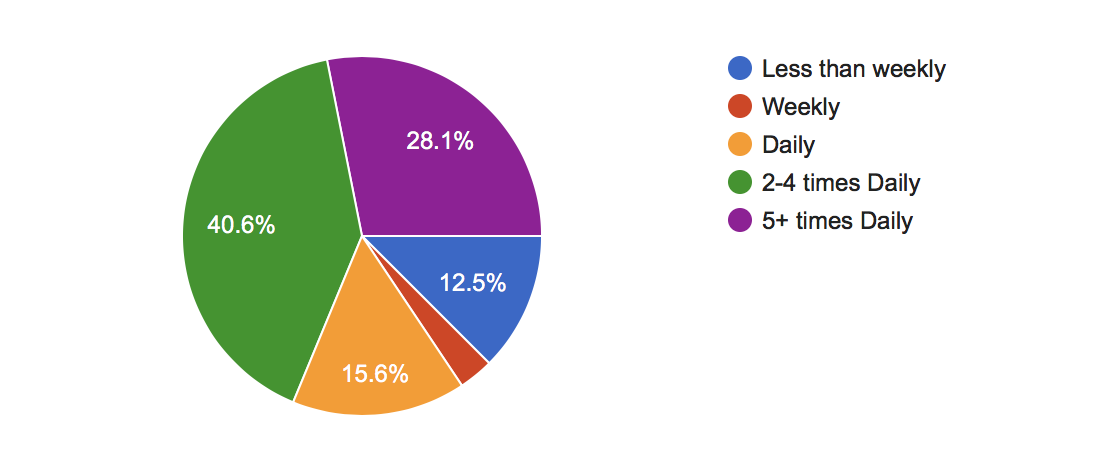
\includegraphics[scale=0.7]{01HowOftenDoYouReadTheNews}
   \caption[Survey Graph surrounding how often news is read]{A pie chart showing how often people read the news.}
   \label{SurveyHowOftenDoYouReadTheNews}
\end{figure}

The first question (Figure \ref{SurveyHowOftenDoYouReadTheNews}) on the survey was designed to ascertain how often people read the news. Overall, well over 80\% of respondents said that they read the news at least daily, and nearly 60\% more than once per day. \\

\item \textbf{How many sources do you read?}

\begin{figure}[ht!]
  \centering
    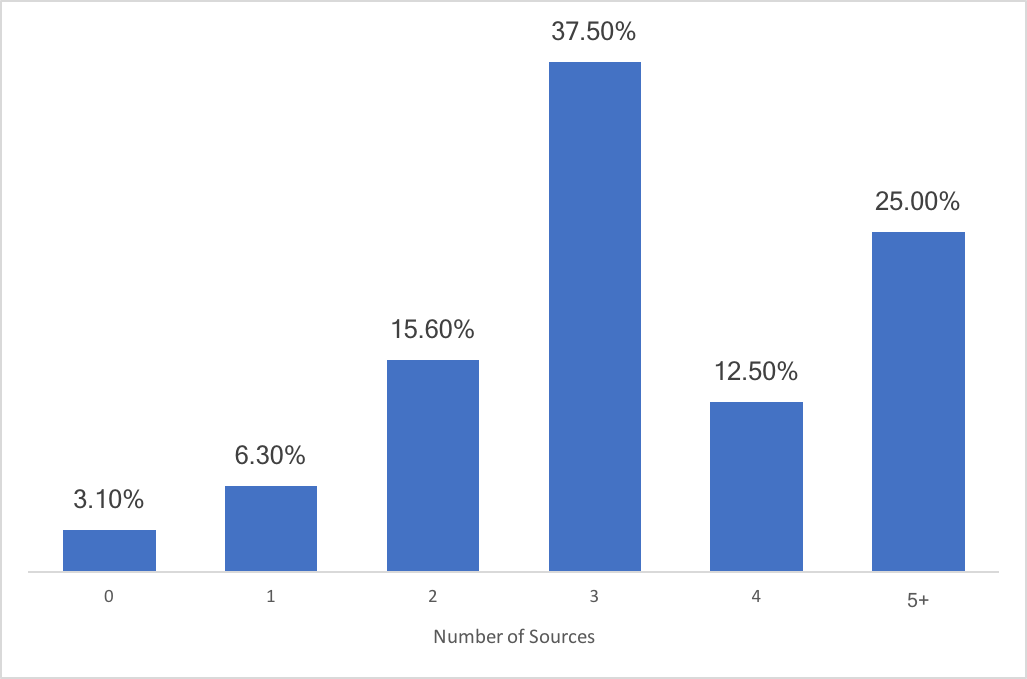
\includegraphics[scale=0.7]{02HowManySourcesDoYouRead}
   \caption[Survey Graph asking how many sources are used]{A bar graph showing how many sources people normally use for a source of news.}
   \label{SurveySources}
\end{figure}

Next I asked about how many sources a user read. It was quite rare for someone to use only one source for a piece of news. In fact, over 90\% said that they used two or more sources, with three and five sources being the most prominent selections. \\

\item \textbf{Are these the same sources every time?}

\begin{figure}[ht!]
  \centering
    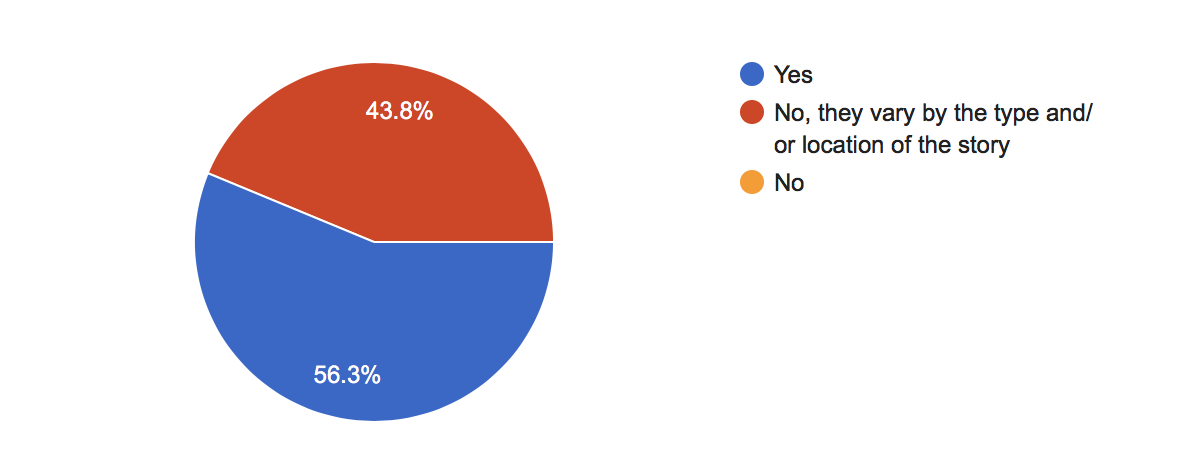
\includegraphics[scale=0.7]{03AreTheseTheSameSourcesEverytime}
   \caption[Survey Graph about consistency of sources]{A pie chart showing whether people use the same sources every time.}
   \label{SurveySourceConsistency}
\end{figure}

The respondents were a lot more split on the question of consistency of sources, although more than half said that they used the same sources every time, with 43.8\% saying that they vary their sources based on the type and/or location of the news story. \\

\item \textbf{How much of an article do you normally read?}

\begin{figure}[ht!]
  \centering
    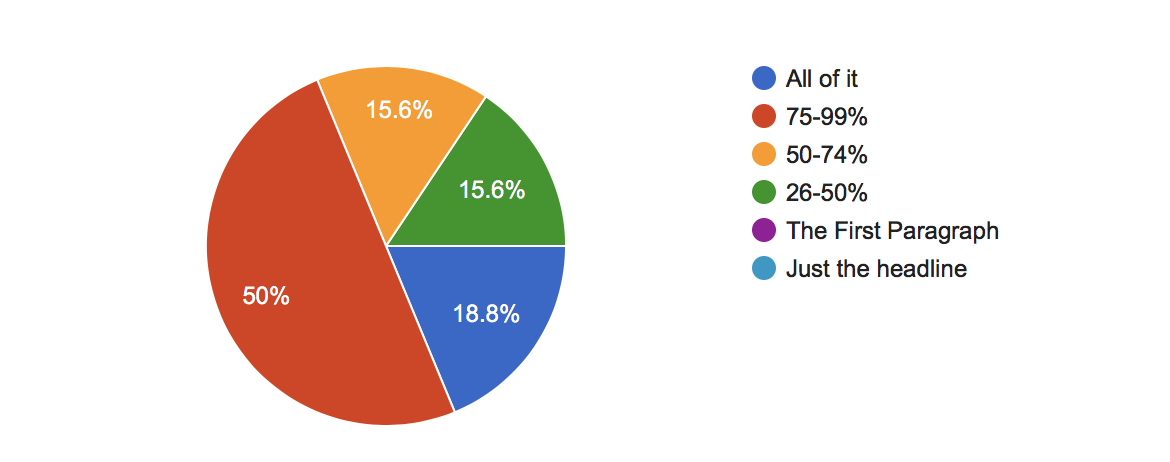
\includegraphics[scale=0.7]{05HowMuchOfAnArticleDoYouRead.png}
   \caption[Survey Graph regarding how much of an article is read]{A pie chart showing how much of articles people normally read.}
   \label{SurveyArticleLength}
\end{figure}

I further expanded upon the initial reading I had done about attention spans by asking potential users how much of articles they normally read. Only 18.8\% of respondents said that they read the entirety of articles (Figure \ref{SurveyArticleLength}), and as much as 15.6\% confess that they read less than 50\% of an article on average. It's plausible that the users could be missing key facts through not reading the entire article. On reflection, I could have also asked if this was a concern to those users. \\

\item \textbf{If an article was presented as a shorter summary, would you read more/all of it?}

\begin{figure}[ht!]
  \centering
    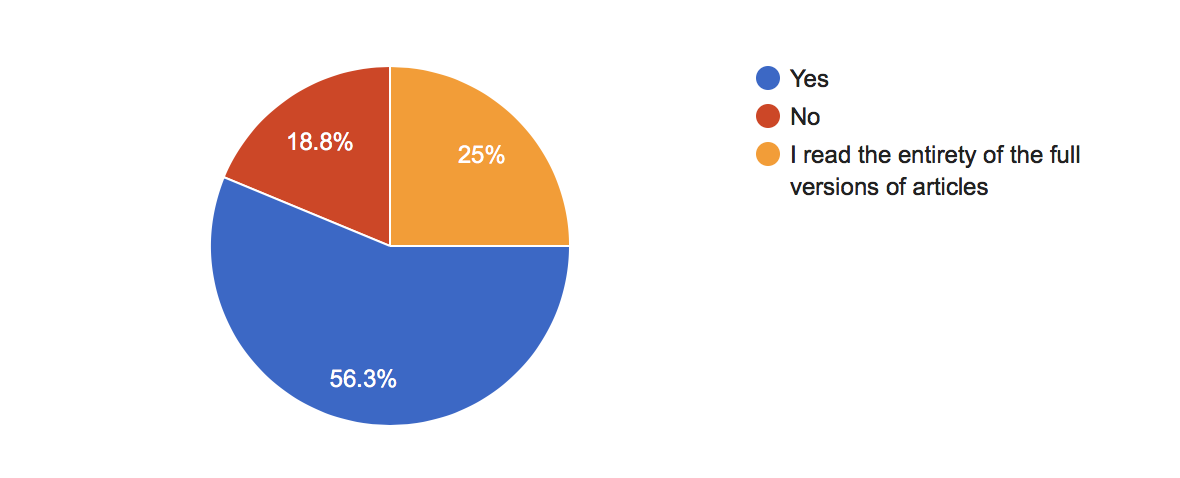
\includegraphics[scale=0.7]{06WouldYouReadAShorterSummary.png}
   \caption[Survey Graph regarding summarisations of articles]{A pie chart showing what percentage of people would read a shorter summary of an article.}
   \label{SurveyArticleLength}
\end{figure}

Another question asked was whether reading a shorter summary would result in users reading more or all of the article. Encouragingly, more than half (56.3\%) of respondents said that they would read a shorter summary. \\

\item \textbf{Would you read a summary of different articles on the same topic combined?}

\begin{figure}[ht!]
  \centering
    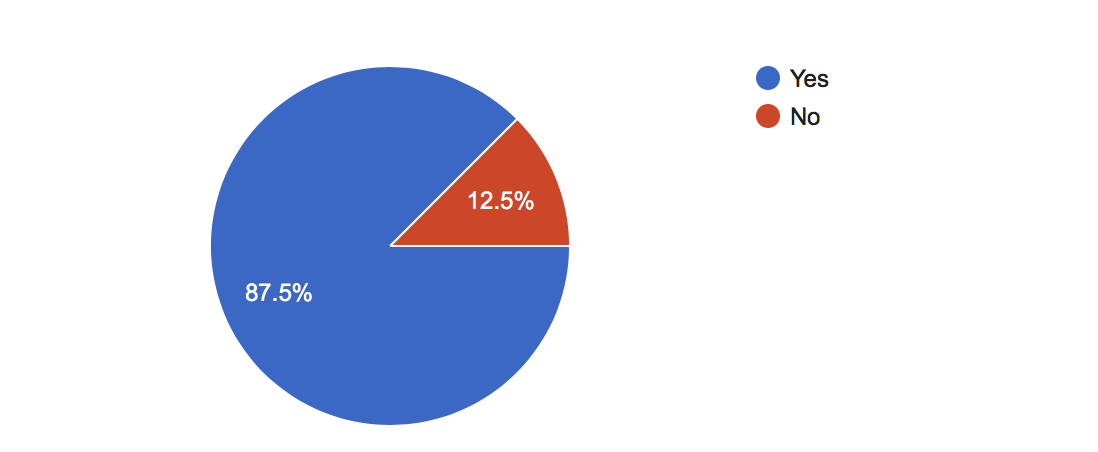
\includegraphics[scale=0.7]{07WouldYouReadASummaryOfArticlesCombined}
   \caption[Survey Graph about combining articles]{A pie chart showing whether people would read a summary of different articles on the same topic combined.}
   \label{SurveySummarisedArticles}
\end{figure}

With this question (Figure \ref{SurveySummarisedArticles}) I aimed to obtain an idea from potential users as to whether combining articles about the same topic from different sources and then summarising it would be considered useful. The question got a resounding response, with as much as 87.5\% saying that they would read a summary like this.  \\

\item \textbf{Would you use a News Aggregator that summarised articles?}

\begin{figure}[ht!]
  \centering
    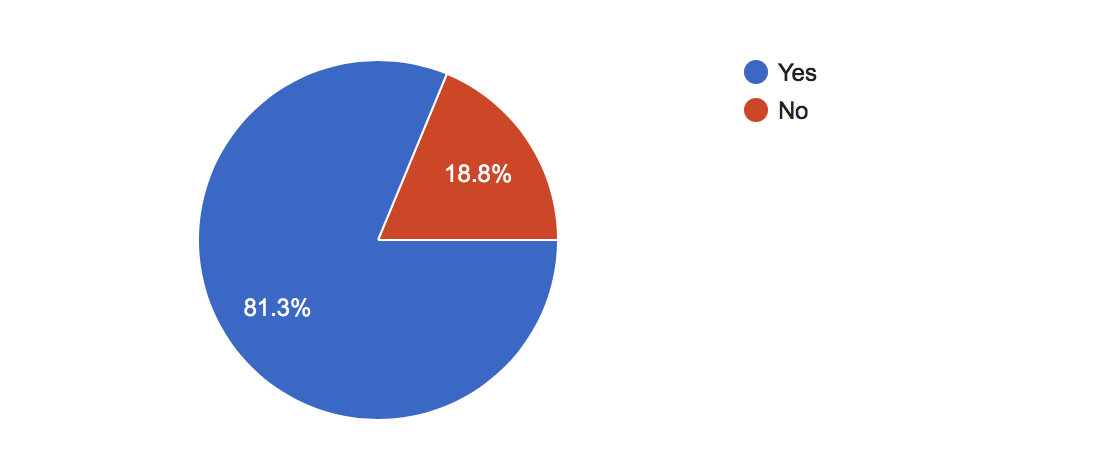
\includegraphics[scale=0.7]{08WouldYouUseANewsAggregatorThatSummarised}
   \caption[Survey Graph concerning News Aggregators and summarisation]{A pie chart showing answers to the question: "Would you use a News Aggregator\index{News Aggregator} that summarised articles"}
  \label{NewsAggregatorThatSummarised}
\end{figure}

Consolidating the findings of the previous question was the fact that 81.3\% said they would use a News Aggregator\index{News Aggregator} that summarised\index{Summarised} articles (Figure \ref{NewsAggregatorThatSummarised}). Amongst those who said they wouldn't, there were comments along the lines of "I'm not great with technology" given as explanation. An interesting comment however, said that "nuance could be lost in the summarisation". This is a valid point, and so a key point of the evaluation\index{Evaluation} process will have to be focused on the summarisation of articles itself, to ensure it's not losing important information at any stage.\\

\item \textbf{How often do you search for news on a specific topic?}

\begin{figure}[ht!]
  \centering
    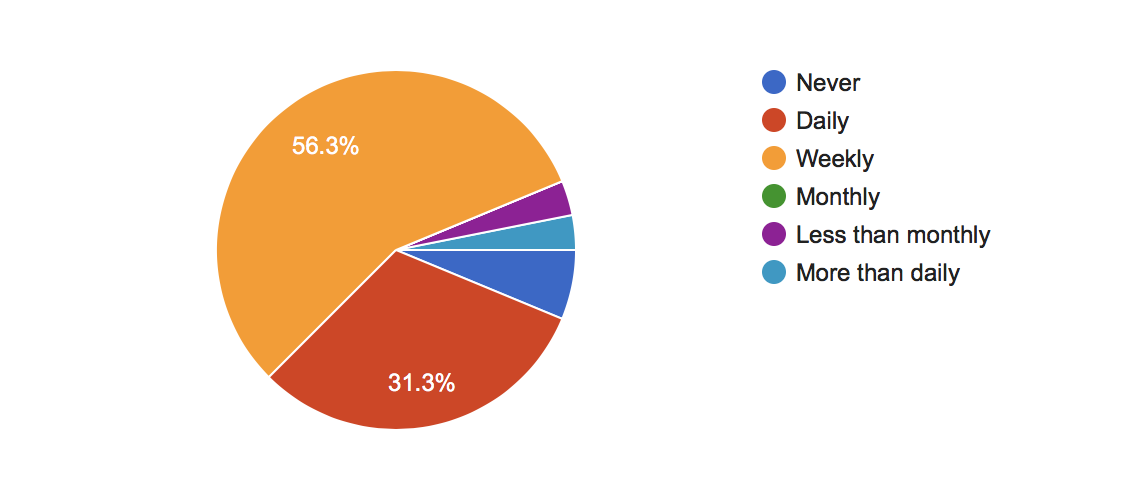
\includegraphics[scale=0.7]{10HowOftenDoYouSearchForASpecificTopic}
   \caption[Survey Graph regarding searching for topics in the news]{A pie chart showing how frequently people search for news on a specific topic.}
   \label{SurveySearchingForTopics}
\end{figure}

For the questions in Figure \ref{SurveySearchingForTopics} I tried to get an idea of how much people search for news on a specific subject of interest to them. In general, this came out to be less frequent then reading the news itself, with just over half the respondents saying that they search for a specific topic weekly. However, a healthy proportion (31.3\%) search daily for specific topics, and some search even more often than this.\\

\item \textbf{Should the news aggregator have the ability to search for a specific topic?}

\begin{figure}[ht!]
  \centering
    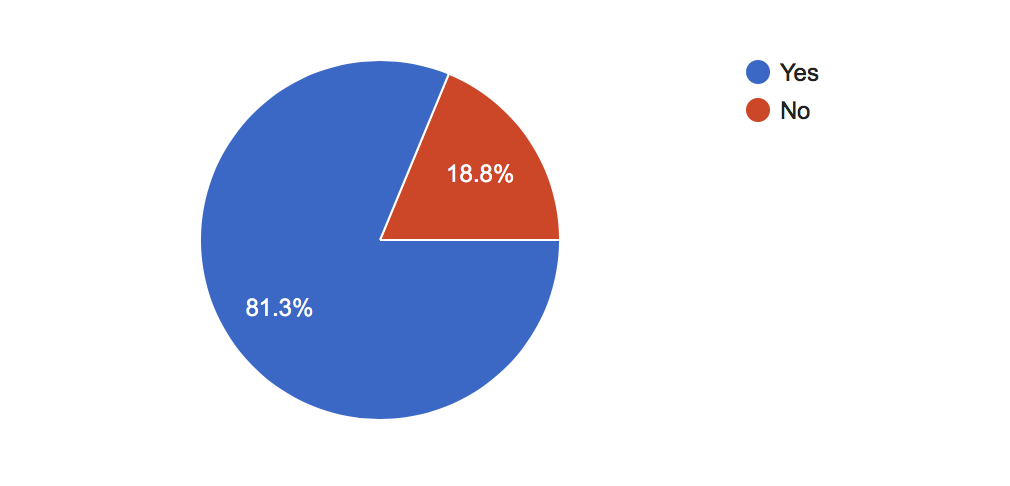
\includegraphics[scale=0.7]{11ShouldNewsAggregatorProvideSearchingForSpecificTopic.png}
   \caption[Survey Graph regarding news aggregators and searching]{The answers to a question asking if the News Aggregator should have the ability to search for a specific topic.}
\end{figure}

As much as 81.3\% of respondents agreed that the News Aggregator\index{News Aggregator} should have a function to search for specific topics. \\

\item \textbf{Do you like services such as news digests that prepare lists of articles each day that apply to a topic you may be interested in?}

\begin{figure}[ht!]
  \centering
    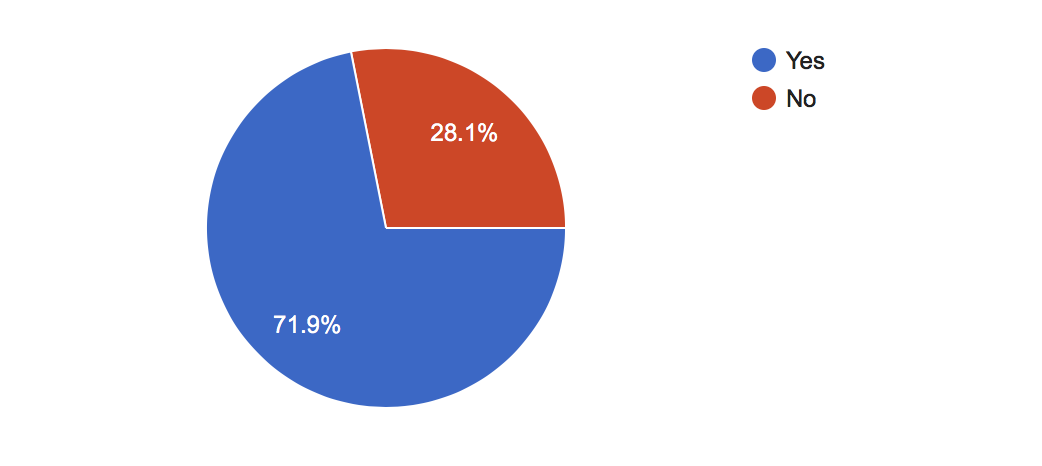
\includegraphics[scale=0.7]{12DoYouLikeServicesThatProduceDigests}
   \caption[Survey Graph about News Digests]{A pie chart showing people's attitudes towards News Digests.}
   \label{SurveyDigests}
\end{figure}

The next question, shown in Figure \ref{SurveyDigests} centred around News Digests\index{News Digests}. Nearly 72\% of respondents said that they liked services that provide news digests.\\

\item \textbf{How often should these news digests be updated?}

\begin{figure}[ht!]
  \centering
    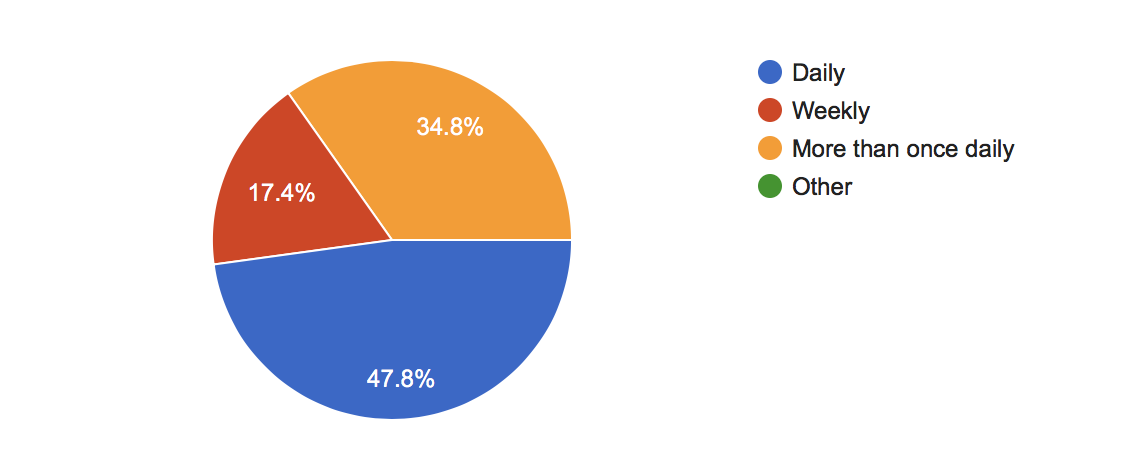
\includegraphics[scale=0.7]{13HowOftenShouldTheseDigestsBeProduced}
   \caption[Survey Graph about News Digests' frequency]{Responses regarding how frequently news digests should be updated.}
\end{figure}

People who were in favour of news digests in general felt that these should be updated at least daily (47.8\%), with a further 34.8\% on top of that saying it should be updated more than once.\\

\item \textbf{What platform should the aggregator be developed for?}

\begin{figure}[ht!]
  \centering
    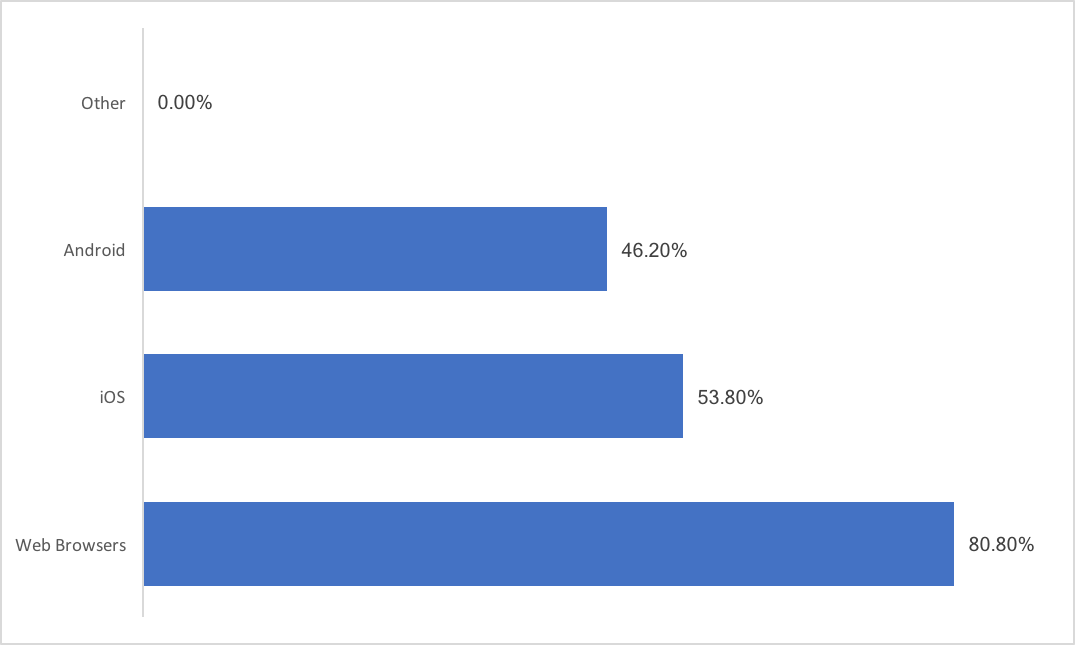
\includegraphics[scale=0.7]{09WhatPlatform.png}
   \caption[Survey Graph concerning potential platforms]{A bar chart showing responses when asked which platform they'd rather see the news aggregator developed for.}
   \label{Survey Platform}
\end{figure}

Finally, respondents were asked which platform they would prefer to see the news aggregator developed for. 80.8\% said they'd want a version for web browsers, and 53.8\% for iOS and 46/2\% for Android. This would suggest that I should develop a web solution and then move to a mobile platform afterwards if there is time.\\

\end{enumerate}
 
\subsection{Related Products}

\subsubsection{Google News}\index{Google!News}

\begin{figure}[H]
  \centering
  \begin{subfigure}{0.8\textwidth}
        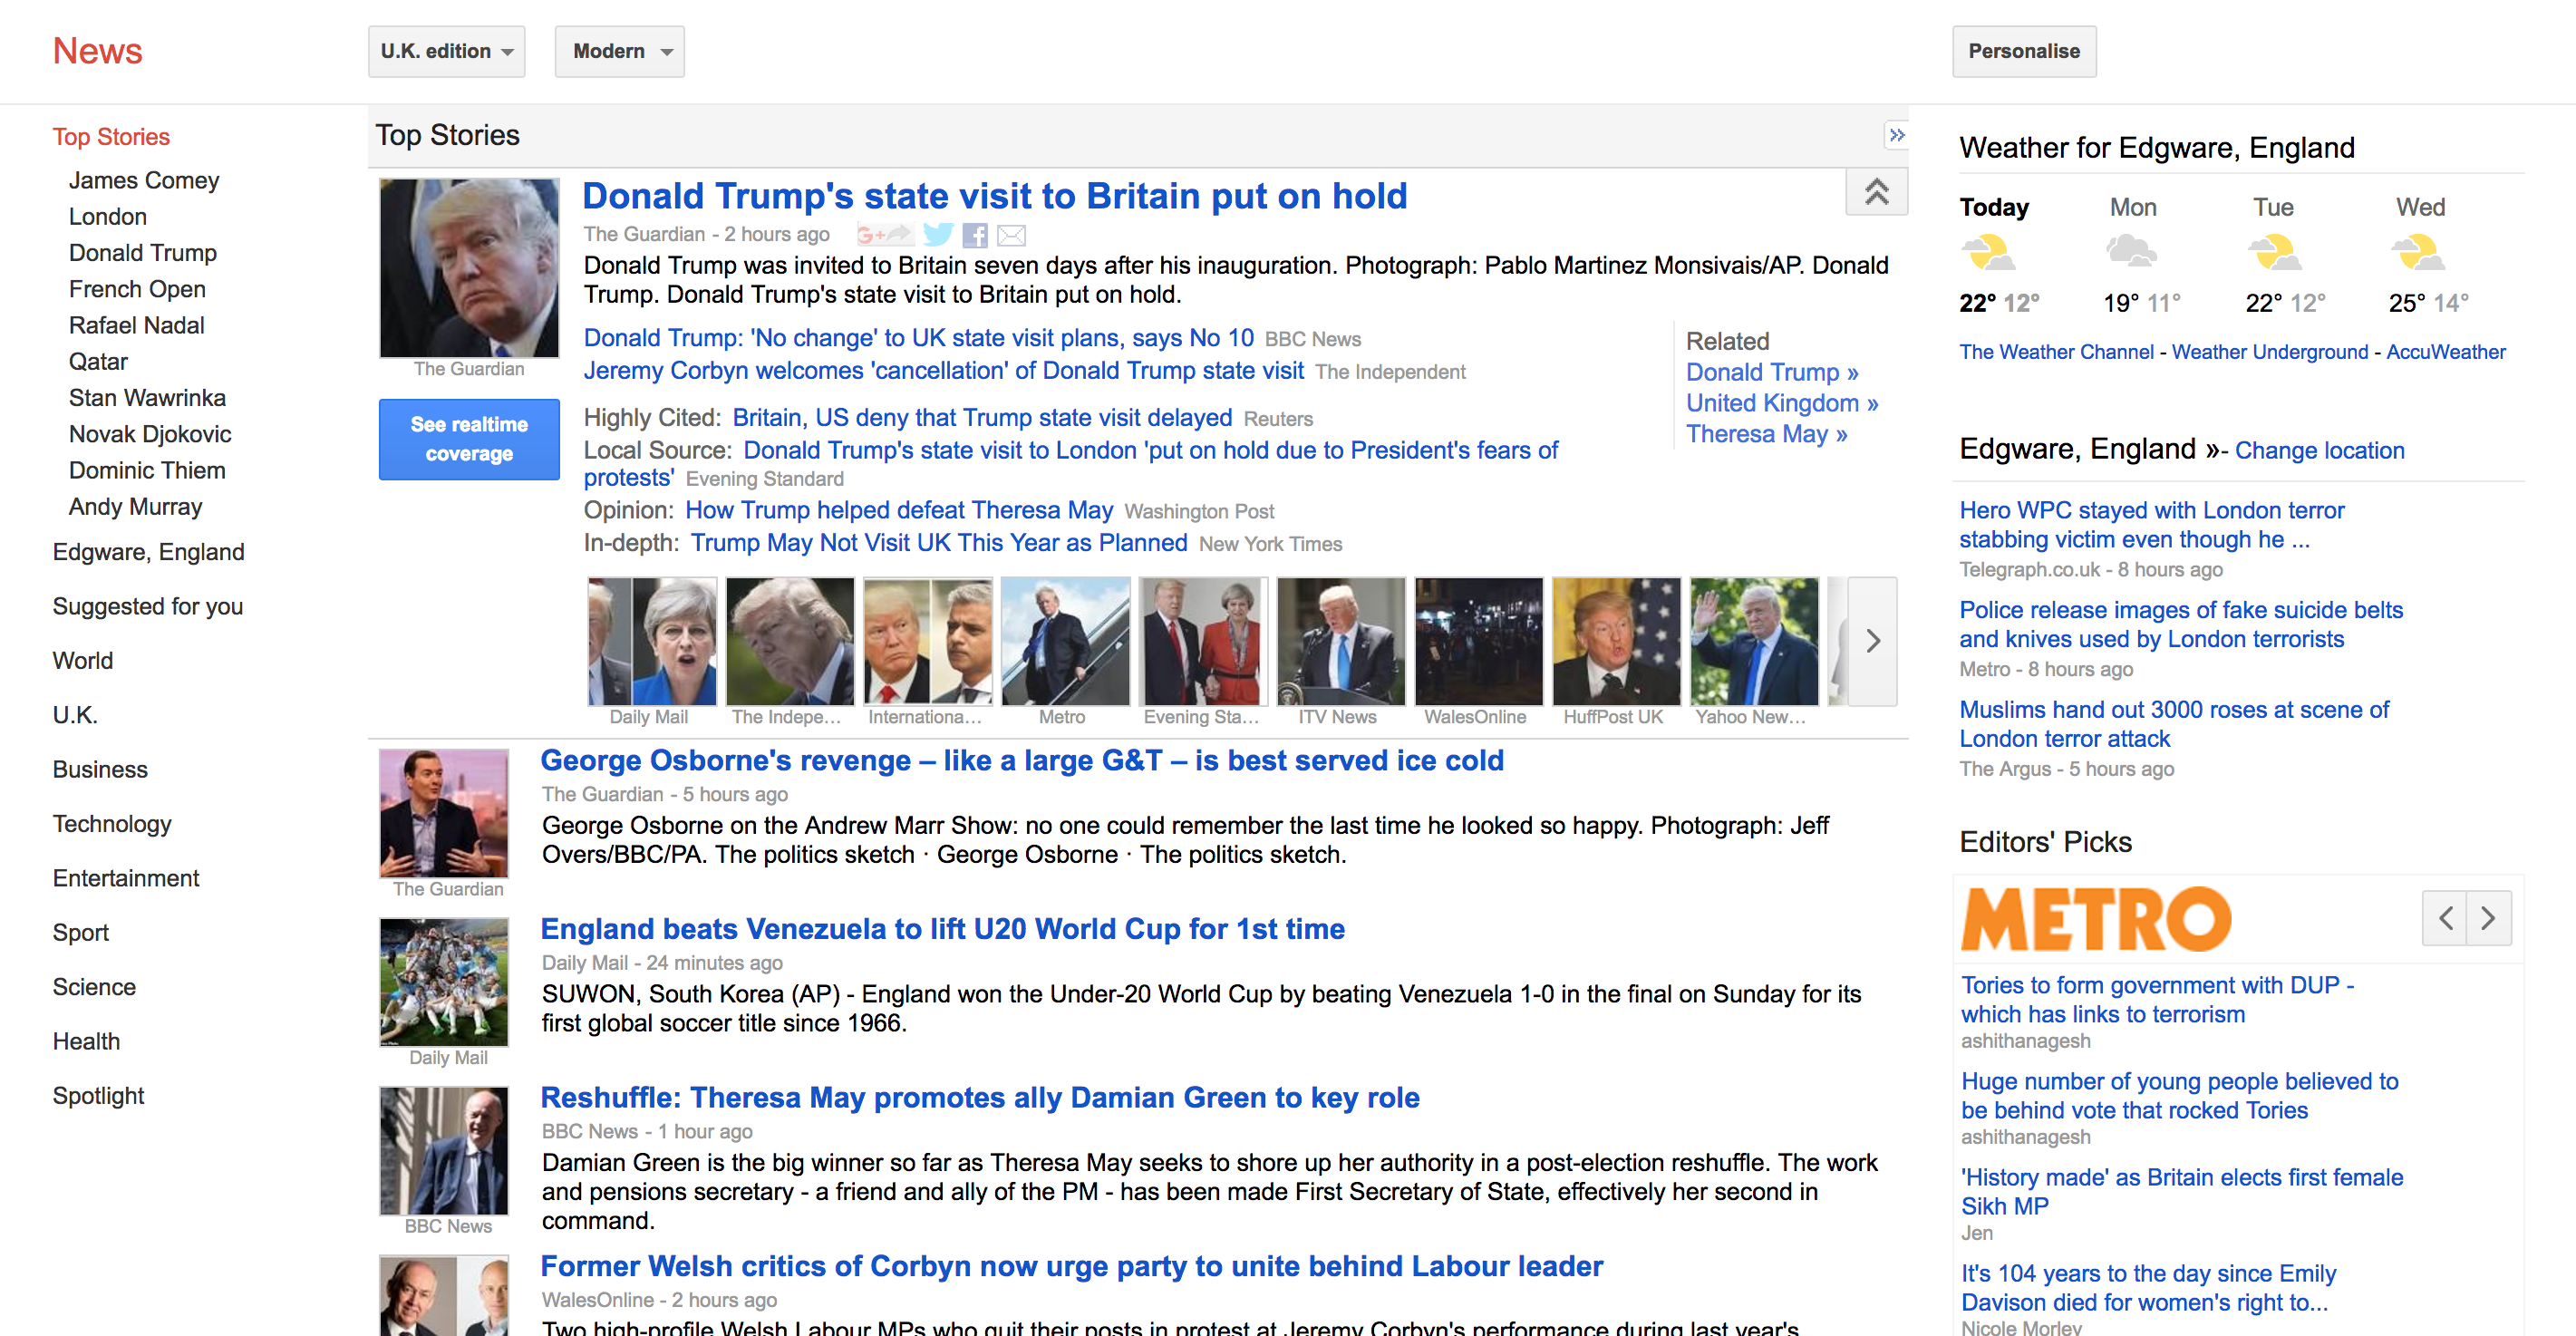
\includegraphics[width=\textwidth]{GoogleHome}
        \caption[Screenshot from the Google News home page]{A section of the homepage for Google News.\cite{googleNews}}
        \label{GoogleNewsHome}
    \end{subfigure}
    
    \begin{subfigure}{\textwidth}
    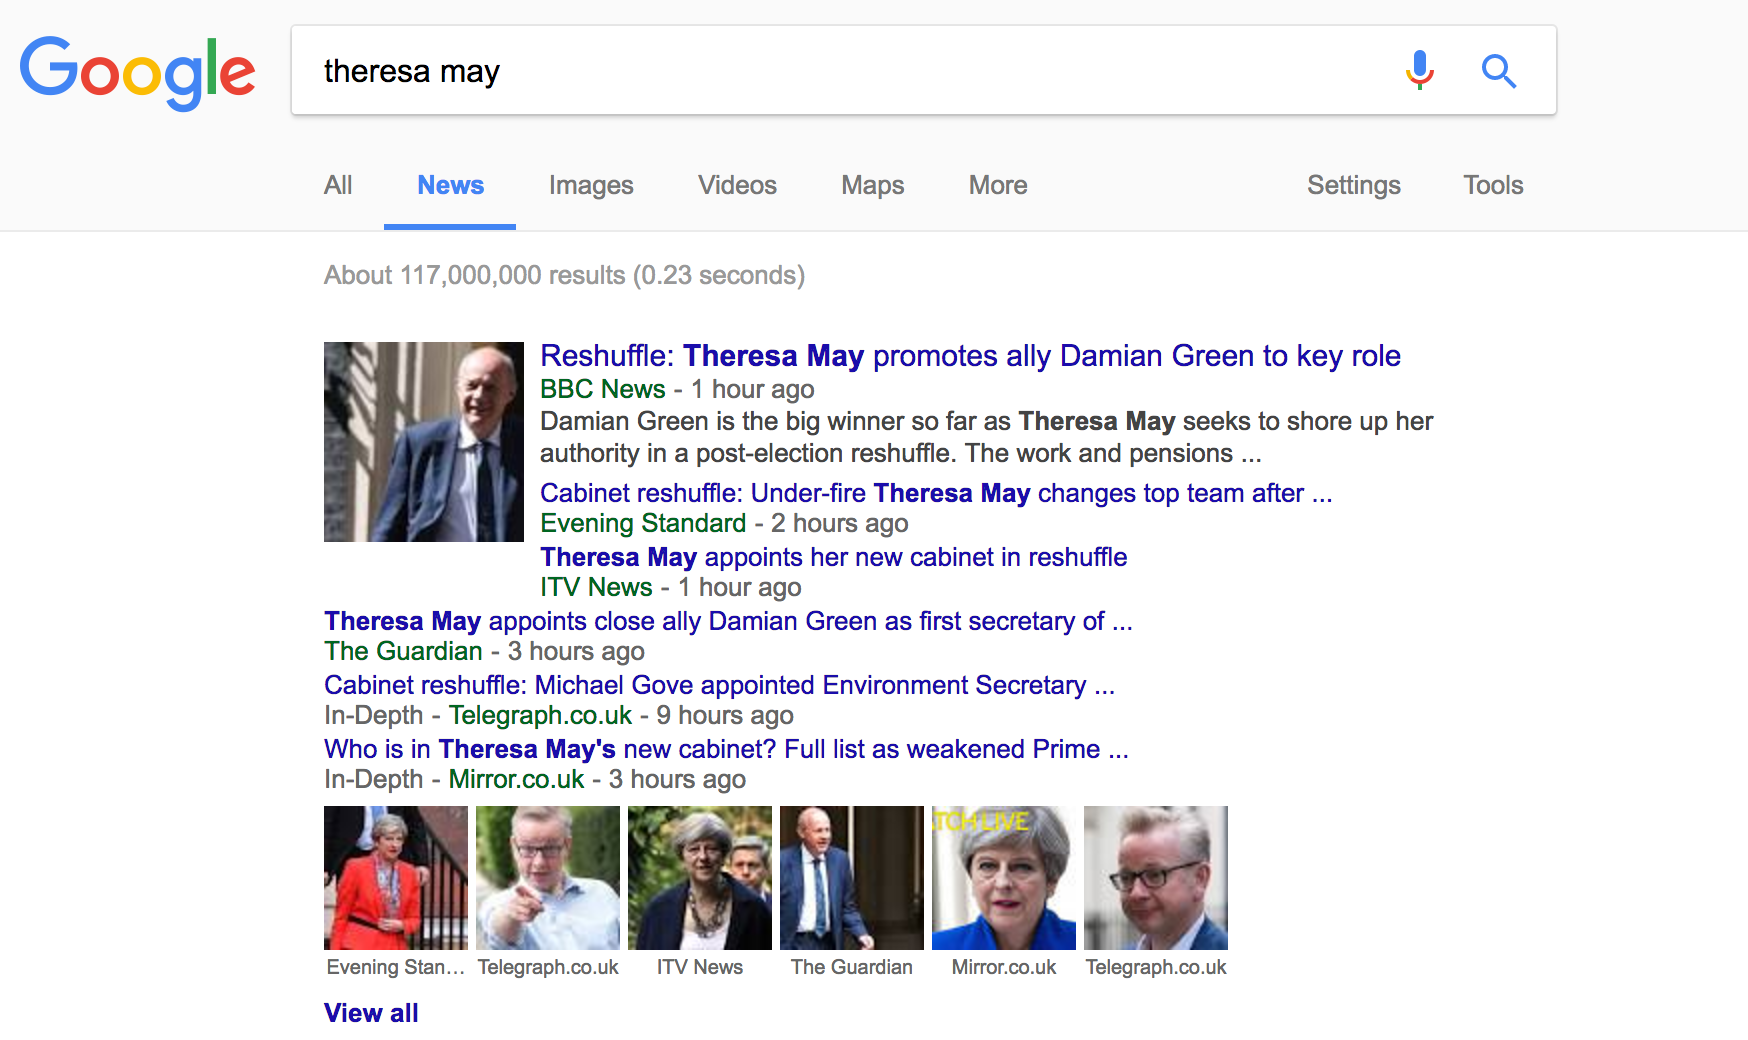
\includegraphics[width=\textwidth]{GoogleUber}
   \caption[Screenshots from a Google News search]{Google News uses clustering techniques to group articles about the same topic together. }
   \label{GoogleNewsUber}
   \end{subfigure}
   \caption[Screenshots from Google News]{Screenshots from Google News}
\end{figure}

Initially developed early in the century and released in 2006, Google News\cite{googleNews} is a free-to-use news aggregator. Google News operates in a similar manner to the traditional Google\cite{google} search engine, thus making it a go to aggregator when searching for a specific topic. Google News also groups "similar" articles together using Clustering\index{Clustering} techniques\cite{googleClustering}. Google News operates purely as a go-between - when clicking on an article the user is taken straight to the media source itself, rather than being able to read the article on Google News itself. 

\subsubsection{Flipboard}\index{Flipboard}

\begin{figure}[H]
  \centering
  \begin{subfigure}[t]{0.3\textwidth}
        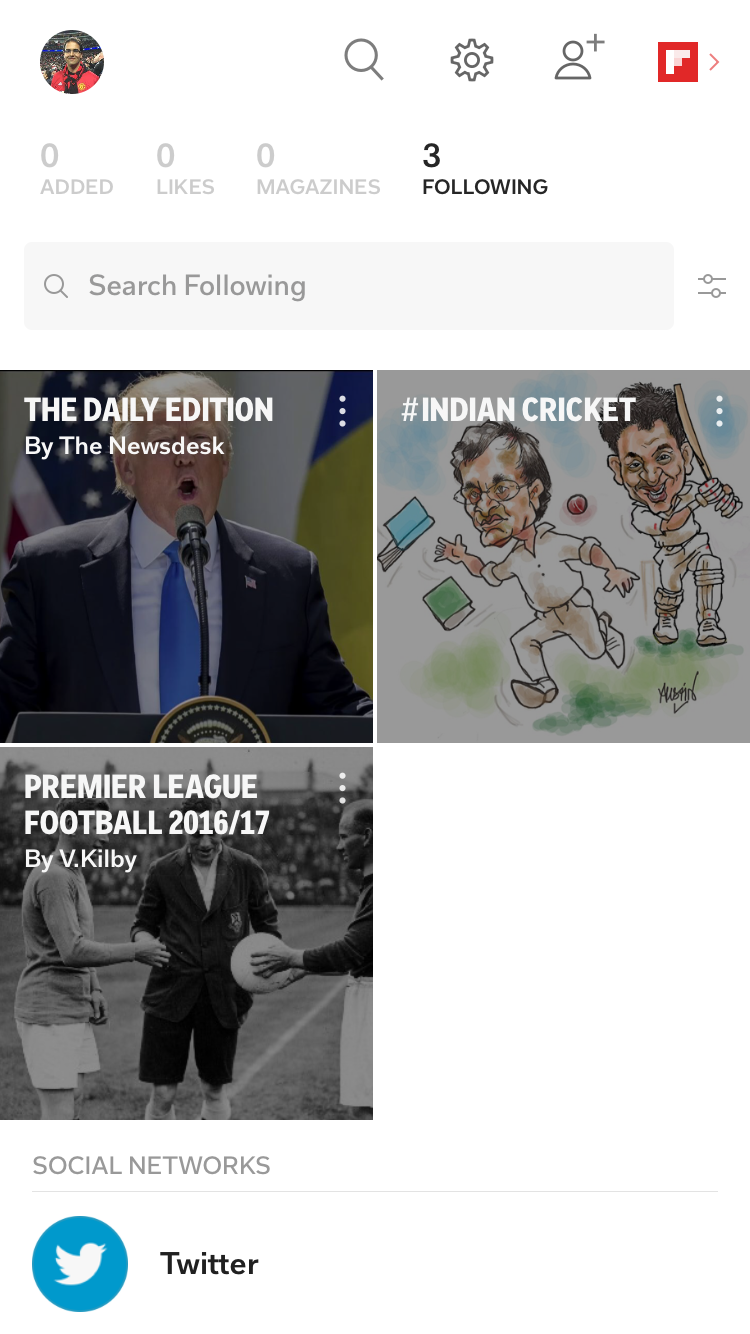
\includegraphics[width=\textwidth]{FlipboardHome.PNG}
        \caption{Users can subscribe to "magazines" that they may be interested in.}
        \label{FlipboardHome}
    \end{subfigure}
    \qquad
    \begin{subfigure}[t]{0.3\textwidth}
    
\includegraphics[width=\textwidth]{Flipboard.PNG}
   \caption{All users are subscribed to \emph{The Daily Edition}, which puts together the latest most popular news.}
   \label{FlipboardDailyEdition}
   \end{subfigure}
   \caption[Screenshots from the Flipboard app]{Screenshots from the Flipboard app}
\end{figure}

Flipboard\cite{flipboard} is a much more recent attempt at a news aggregator (developed in 2010), and relies on the concept of users subscribing to "magazines" on different topics. There's a central "cover page" on the home page that shows the most recent stories from across all a user's subscriptions. Like Google News\index{Google!News}, links from the desktop website send the user to the original media source, while links from within the mobile applications open a browser within the app itself.

\subsubsection{Yahoo News Digest}\index{Yahoo News Digest}

\begin{figure}[ht!]
  \centering
  \begin{subfigure}[t]{0.3\textwidth}
        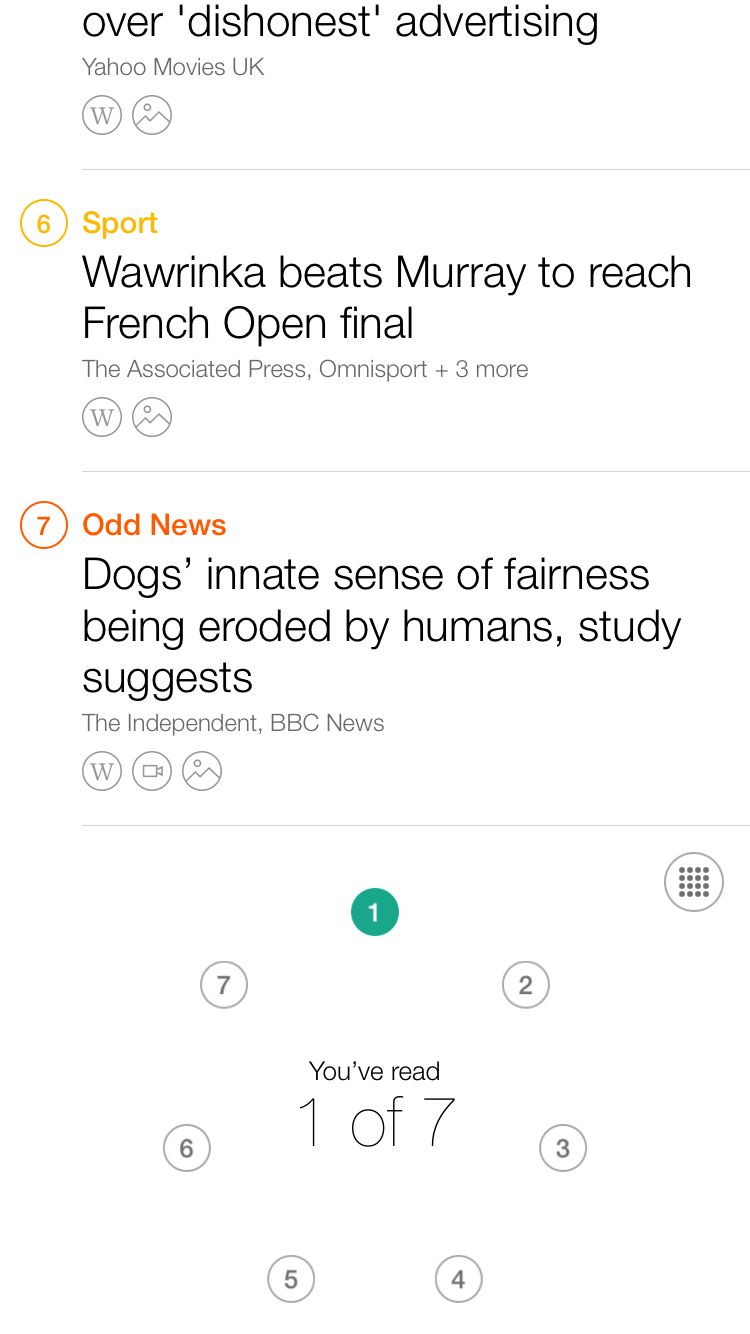
\includegraphics[width=\textwidth]{YNDHome.PNG}
        \caption{A section of the home screen, which displays the top ten stories for the day.}
        \label{YNDHome}
    \end{subfigure}
    \qquad
    \begin{subfigure}[t]{0.3\textwidth}
    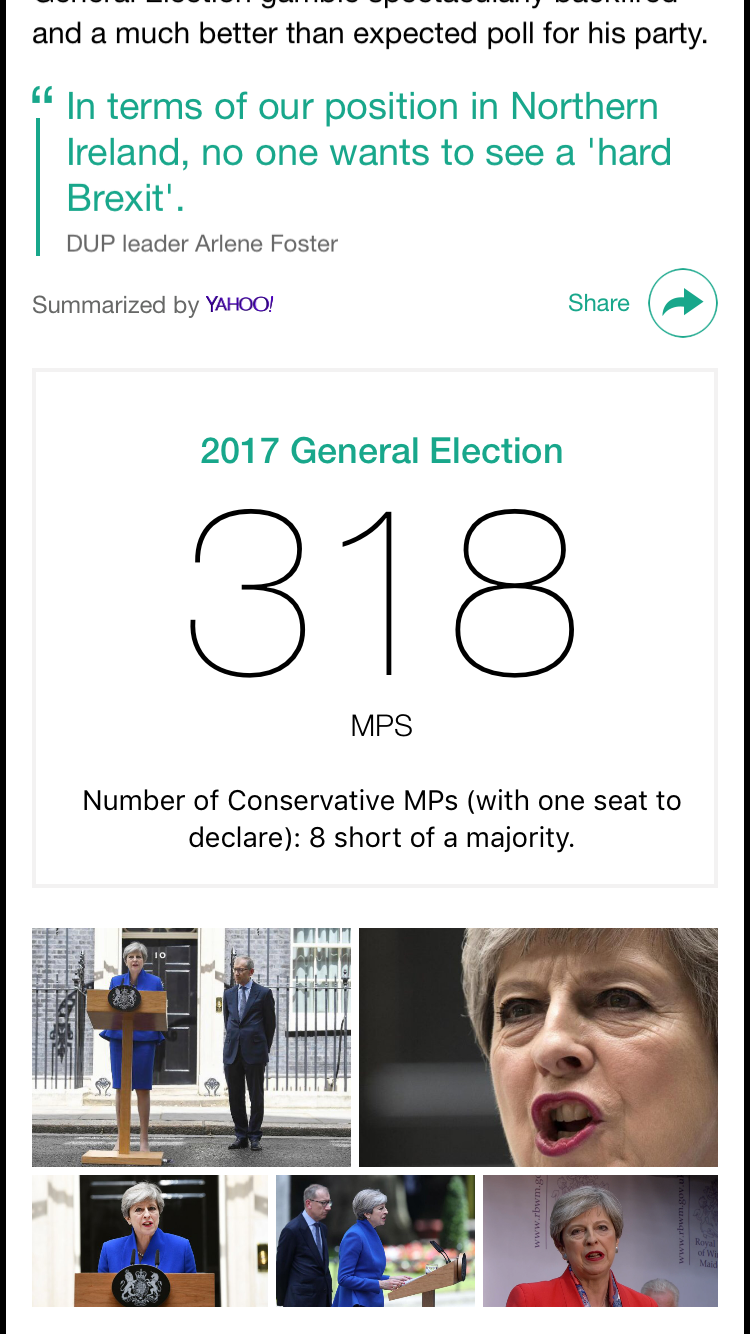
\includegraphics[width=\textwidth]{YNDInfo.PNG}
   \caption{The Yahoo News Digest app provides links and infographics that are relevant to the article.}
   \label{YNDInfo}
   \end{subfigure}
   \caption[Screenshots from the Yahoo News Digest app]{Screenshots from the Yahoo News Digest app\cite{yahooNewsDigest}}
\end{figure}

Yahoo News Digest\cite{yahooNewsDigest} is a direct evolution from Summly\cite{summly}, which was an app that summarised news. Yahoo News Digest is a phone application that creates two digests a day: one in the morning and one in the evening. Each digest contains the ten leading articles from the previous 12 hours. Each article provides a summary of the story and links to relevant other pages - such as articles from Wikipedia\cite{wikipedia}.

\subsubsection{Apple News}\index{Apple!News}

\begin{figure}[ht!]
  \centering
  \begin{subfigure}[t]{0.3\textwidth}
        
\includegraphics[width=\textwidth]{AppleHome.PNG}
        \caption{The home screen for the Apple News app}
        \label{AppleHome}
    \end{subfigure}
    \qquad
    \begin{subfigure}[t]{0.3\textwidth}
    
\includegraphics[width=\textwidth]{AppleSources.PNG}
   \caption{Apple News allows users to select sources and topics to be their favourites.}
   \label{AppleSources}
   \end{subfigure}
   \caption[Screenshots from the Apple News app]{Screenshots from the Apple News app\cite{appleNews}.}
\end{figure}

Apple News\cite{appleNews} is an application that is installed by default on all recent iOS devices. Apple's default attempt at a news aggregator allows users to select their preferred news sources, and from a selection of topics. Apple\cite{apple} then presents on a home screen news from those sources and topics. Clicking on each article keeps it in the native application, rather than sending the user to the media source itself.

\subsubsection{Comparing the existing products}

The existing products are compared in Table \ref{relatedProductsTable} on page \pageref{relatedProductsTable}.

\begin{sidewaystable}
    \begin{tabular}{p{2.5cm}|p{8.75cm}|p{8.75cm}}
    \textbf{Product} & \textbf{What it does well} & \textbf{What it doesn't do well} \\ \hline
    Google News & \tabitem Groups similar articles together & \tabitem Doesn\'t host articles itself - therefore making it harder to navigate than perhaps could be possible. Although, this could be to avoid any copyright issues. \\ & \tabitem Similar to a traditional search engine and so is easy to use\\ & \tabitem Obtains articles instantly, thus providing most up-to-date information when searching  \\ \hline
    Flipboard & \tabitem Provides a home page that allows a user to see the most popular stories at the time related to the user's subscriptions. & \tabitem Topics are much broader than Google News, thus meaning that users can't necessarily search for topics specific-enough for them.\\ & \tabitem Available as a mobile application & \tabitem Flipboard requires registration before being able to read articles \\ \hline
    Yahoo News Digest & \tabitem Yahoo News Digest won the 2014 Apple\index{Apple} Design award\cite{appleDesignAward}\index{Apple!Design award}. & \tabitem There are only ten articles available per digest, and no capability for searching by topic. \\ & \tabitem The articles also provide key infographics, quotes, and other information potentially relevant to the article. & \tabitem Digests are only produced in the morning and the evening, so the news articles presented could be out of date. \\ \hline
    Apple News & \tabitem Allows selection based off both topics and the news sources themselves. & \tabitem Navigation on the application is not simple. If a user has accessed many articles from push notifications, then the user could have to press the back button several times to get back to the home screen.\\ & \tabitem The home screen for the app allows users to see a lot of headlines at a glance. & \tabitem The topics that a user can subscribe to can be quite limited, and aren't reactive to current affairs - for example, if a natural disaster occurs, you couldn't then subscribe to that natural disaster as a topic. \\
  \end{tabular}
  \caption[Related Products in the market and their benefits and drawbacks]{Comparing the relative benefits and drawbacks of Google News, Flipboard, Yahoo News Digest and Apple News}
  \label{relatedProductsTable}
\end{sidewaystable}

%%%%%%%%%%%%%%%%%%%%%%%%%%%%%%%%%%%%%%%%%%%%%%%%%%%%%%%%%%%%%%%%%%%%%%%%%%%%%%%%%%%%%%%%%%

\pagebreak

\section{Background Research}

\subsection{Machine Learning Techniques}

\subsubsection{Topic Modelling Techniques}\index{Topic Modelling}

\label{TopicModellingTechniques}

Topic modelling is a subsection of Machine Learning\index{Machine Learning} that aims to determine what topic a given document is about. The topics wouldn't be named at this stage, they would simply be given generic names such as Topic A and Topic B. Assigning names to topics will be done at a later stage (see Section \ref{TopicLabelingTechniques}).

\textbf{Latent Semantic Indexing}\index{Latent Semantic Indexing}\index{Topic Modelling!Latent Semantic Indexing}

Also known as Latent Semantic Analysis\index{Latent Semantic Analysis}\cite{lsa}, Latent Semantic Indexing (LSI) was one of the initial forerunners in the field of topic modelling. It uses singular value decomposition to locate patterns in the text of a document and thus form a basis on which to categorise the document. A major benefit of LSI\index{LSI} is that it is fast to train, but in general it has lower accuracy when compared to models that are probabilistic, such as Latent Dirichlet Allocation\index{Latent Dirichlet Allocation}\cite{differenceBetweenLSIAndLDA}.

\textbf{Latent Dirichlet Allocation}

Latent Dirichlet Allocation\index{Latent Dirichlet Allocation} (LDA)\index{LDA}\index{Topic Modelling!Latent Dirichlet Allocation} is a generative probablistic model that assumes that the topic distribution has a Dirichlet prior. The theory behind LDA is that a document of words contains a mixture of different topics, and this is reflected in the final answers given for the algorithm.

\emph{A rough algorithm for performing LDA\cite{ldaExplanation}:}

\begin{enumerate}
	\item \textbf{Set \emph{n} to be the number of topics there are in the document.} We can do this by trial and error. \\
	\item \textbf{Assign every word \emph{w} in the document {d} to a random topic.} These topics are temporary. At this stage we can remove function words, such as "the". However, we keep duplicates - in fact, at this stage they could be in different topics. \\
	\item \textbf{Check and update topic assignments.} To do this, we loop through each word in the document, taking note of how prevalent the word is across documents, and prevalent those topics are in the document. These two probabilities are then passed to a sampling algorithm to generate a new topic for the word. This step is usually completed using the statistical model \emph{Gibbs Sampling}\index{Gibbs Sampling}.
	\item \textbf{Repeat step 3 until there are no more topic-reassignments}. 
\end{enumerate}

\subsubsection{Topic Labelling Techniques}\index{Topic Labelling}

Topic Labelling techniques in the project for labelling the topics that are generated from the LDA analysis of the document in Section \ref{TopicModellingTechniques}. When conducting research into this topic specifically, I found a paper (\emph{Automatic Labelling of Topic Models}\index{Automatic Labelling of Topic Models} by Lau, Grieser, Newman and Baldwin in 2011\cite{topicLabelling}) that documents the creation of an algorithm that labels topics using Wikipedia\cite{wikipedia}\index{Wikipedia} titles. This could work very well in my project, as Wikipedia titles as title headings would allow users to search for topics that are both broad and specific. 

\emph{A rough version of Lau, Grieser, Newman and Baldwin's algorithm:}

\label{labellingalgorithm}

\begin{enumerate}
	\item \textbf{Calculate the top 10 topic terms.} This is done by finding the marginal probabilities of each word from the original topic models, and taking the top ten. The marginal probability of a term is the probability of that term being randomly selected given a topic \emph{t}. \\
	\item \textbf{Search Wikipedia\index{Wikipedia} using these terms.} We also search Google\cite{google}\index{Google} using a site restricted search (to Wikipedia) and take the top eight results from each. These are called the \emph{primary labels}. \\
	\item \textbf{Isolate all "noun chunks" from the terms.} In this case noun chunks are combinations of words from the terms that appear next to each other. For example, with the term "Summer Olympic Games" the noun chunks would be "Summer", "Olympic", "Games", "Summer Olympic", "Olympic Games" and "Summer Olympic Games". Note that "Summer Games" is not a noun chunk as the words don't appear juxtaposed. These noun chunks are added to the primary labels from step 2 and are deemed \emph{secondary labels}. \\
	\item \textbf{For each noun chunk:} 
		\begin{itemize}
			\item Check to see if the noun chunk is the title for a Wikipedia article
			\item Remove the noun chunk if it doesn't correspond to a Wikipedia article\\
		\end{itemize}
		
	\item \textbf{Calculate the \emph{Related Article Conceptual Overlap}\index{Related Article Conceptual Overlap} scores.} Related Article Conceptual Overlap (RACO), developed by Grieser et al in 2011\cite{racoCalculation},  is a calculation designed to identify the strength of relationship between terms by inspecting the category overlap between the terms' corresponding articles. We do this for each secondary label still remaining - details on how to calculate the RACO scores are explained in further detail below. \\
	\item \textbf{Discard all secondary labels with RACO\index{Related Article Conceptual Overlap}  score of less than 0.1.} \\
	\item \textbf{Add five highest topic terms to the list.} Now we return to the original list of topic terms from step 1 and add the five highest to the remaining candidates. \\
	\item \textbf{Perform candidate ranking.} There are multiple ways to do this, but the original paper recommends using a variety of statistical methods, based around a T-test, the Chi-squared test and a log-likelihood test. The aim is to estimate how closely related the candidate is to all the terms in the topic. We then take the top candidate as our final answer. \\
\end{enumerate}

\textbf{Calculating the \emph{Related Article Conceptual Overlap}\index{Related Article Conceptual Overlap} }

\label{RACOcalculation}

\emph{Related Article Conceptual Overlap\index{Related Article Conceptual Overlap} } (RACO) was first introduced as a concept in the paper \emph{Using Ontological and Document Similarity to Estimate Museum Exhibit Relatedness}\cite{racoCalculation} \index{Using Ontological and Document Similarity to Estimate Museum Exhibit Relatedness}by Grieser, Baldwin, Bohnert and Sonenberg in 2011. It compares two terms and estimates their similarity by comparing the two terms' similarity on Wikipedia. The core calculation for RACO goes as follows: 
\[Category-Overlap(a,b) = \left|
\left(\bigcup_{p \in O(a)} C(p)\right) \bigcap \left(\bigcup_{p \in O(b)} C(p)\right)\right|
\]

In this equation, \emph{O(a)} represents the outlinks (the links to other articles from the Wikipedia\index{Wikipedia} article) of an article \emph{a} and \emph{C(p)} represents the set of categories that article \emph{p} is a part of.

An issue with the Category-Overlap calculation as it is, is that there's a bias for articles that are larger than others as they will have more outlinks but won't necessarily be in more categories. As a result it's normalised using Dice's coefficient \index{Dice's coefficient} to produce the final RACO equation:

\[sim_{RACO}(a,b) = \frac{2 \times \left|
\left(\bigcup_{p \in O(a)} C(p)\right) \bigcap \left(\bigcup_{p \in O(b)} C(p)\right)\right|}
{\left(\bigcup_{p \in O(a)} C(p)\right) + \left(\bigcup_{p \in O(b)} C(p)\right)}
\]

\label{TopicLabelingTechniques}

\subsubsection{Clustering Techniques}\index{Clustering}

\label{ClusteringTechniques}

Cluster analysis is a machine learning technique that is used to put items that are similar to each other into groups. In practice it's used by Google News\cite{googleNews} to put articles about the same topic together for a user\cite{googleClustering}. There are multiple commonly used types of cluster analysis: \\

\textbf{Centroid Clustering}\index{Centroid Clustering}\index{Clustering!Centroid}

In Centroid Clustering\cite{clusteringWikipedia}, also known as k-means clustering\index{Clustering!k-means}, there are \emph{k} clusters. A vector is calculated for each article in the list. The article is then assigned to the cluster that is closest to it's vector score. A major downside to this method however is that it requires \emph{k} to be defined in advance. In the context of this project, that's not applicable as we don't know how many different articles we are clustering based on. \\

\textbf{Density Clustering}\index{Density Clustering}\index{Clustering!Density}

Density Clustering\cite{clusteringWikipedia} also involves calculating a vector score for each article. Once these have been calculated, they can be graphed, and the areas of the graph that have highest density are chosen as the clusters. An advantage of this over the centroid clustering methods is that we don't need to know the number of clusters beforehand. However, density clustering can become less accurate as it requires areas of sparse density on the graph to precisely separate the different groups, which isn't always possible. \\

\textbf{Hierarchical Clustering}\index{Hierarchical Clustering}\index{Clustering!Hierarchical}

Hierarchical Clustering\cite{hierarchicalClustering}, which is also known as Connectivity Clustering\index{Clustering}\index{Connectivity}, is based on the idea of using distance measures between articles to identify which ones are most similar. There are two approaches to Hierarchical Clustering: 
 \begin{itemize}
 	\item \emph{Agglomerative}\index{Hierarchical Clustering!Agglomerative}, which is a bottom-up approach, assigns each item to its own cluster and then merges pairs that are closer together. 
	\item \emph{Divisive}\index{Hierarchical Clustering!Divisive}, a top-down approach, that begins with all items in a single cluster, and then proceeds to split it into multiple clusters. \\
\end{itemize}

\textbf{Creating a vector score for each item}

The first step in each of the three clustering techniques is to create a vector score for each item. As this will play a big part in the final results, it's important to get this stage right. This can be split into two steps: \\

\begin{enumerate}
	\item \textbf{Find definitive terms within the article.} This can be done using techniques such as the popular \emph{Term Frequency-Inverse Document Frequency}\index{Term Frequency-Inverse Document Frequency}  (TF-IDF)\index{TF-IDF} , which is explained in further detail below. Proper nouns would be useful in this step, as they are more likely to be relevant to what the article is specifically about. \\
	\item \textbf{Create a vector.} This vector, based from the definitive terms from the first step, would be a set of keywords and corresponding weights. \\
\end{enumerate}

\textbf{Term Frequency-Inverse Document Frequency}\index{Term Frequency-Inverse Document Frequency}

TF-IDF\cite{tfidf} is designed to identify terms that appear frequently in one article that don't occur a lot over the entire set of articles (also known as the \emph{corpus}). Variations of it are commonly used by search engines to identify search results that are most relevant to a query. The calculation for TF-IDF is as follows: \\

\emph{Term Frequency}\index{Term Frequency-Inverse Document Frequency!Term Frequency}

Term Frequency can be most simply calculated as the frequency of a term in a document. However, this could result in a bias towards terms that appear in longer articles. A more accepted way to calculate the Term Frequency therefore is to use a normalising function, called augmented frequency:

\[tf(t,d) = 0.5 + 0.5 \times \frac{f_{t,d}}{max\{f_{t',d} : t' \in d\}} \] \\

\emph{Inverse Document Frequency}\index{Term Frequency-Inverse Document Frequency!Inverse Document Frequency}

Inverse Document Frequency is used to check in how many documents of a corpus \emph{D} a given term \emph{t} occurs. It is an inverse function, so as to minimise the value for the term when it is common amongst various different documents. It is also logarithmically scaled. It is calculated using the following formula:

\[idf(t,D) = \log{\frac{\left|D\right|}{\left|d \in D : t \in d\right|}} \] \\

\emph{Term Frequency-Inverse Document Frequency}\index{Term Frequency-Inverse Document Frequency}

\[tfidf(t,d,D) = tf(t,d) \times idf(t,D)\] 

\subsection{Summarisation Techniques}       

Summarisation\index{Summarisation} techniques will be (predictably) used for summarising the merged articles that were identified by the processes of Topic Modelling \index{Topic Modelling}, Topic Labelling\index{Topic Labelling} and Clustering\index{Clustering}. There are two types of summarisation: 

\begin{itemize}
	\item \textbf{Extractive Summarisation}\index{Summarisation!Extractive}, which consists of taking sentences that are important from the original text, and discarding the rest.\cite{extractiveTechniques}
	\item \textbf{Abstractive Summarisation}\index{Summarisation!Abstractive}, which aims to generate a piece of text using natural language techniques. A key to this is that some words in the final summary may not have been the original piece of text.
\end{itemize}

\subsubsection{Extractive Summarisation Techniques}

\label{extractiveSummarisation}

\textbf{LexRank and TextRank}\index{LexRank}\index{TextRank}

There are two well known examples of extractive summarisation: LexRank and TextRank.

LexRank and TextRank have very similar methods for extracting a summary\cite{lexRank}. Initially a graph is constructed, that consists of one node for each sentence in the corpus. Then a clustering algorithm is applied, using a TF-IDF\index{TF-IDF} calculation to determine similarities. 

There are a couple of key differences between LexRank and TextRank. The first arises in the calculation. Both use a TF-IDF calculation, but they are varied slightly. LexRank uses a cosine similarity function in order to weight the final calculation, whereas TextRank uses a more simple logarithmic weighting to perform the calculation. 

Both use Google's famous PageRank\index{PageRank} algorithm to then rank the importance of each sentence based on the calculations in the previous step. With \emph{d} being a damping factor, the PageRank of a node \emph{u} is given as:

\[p(u) = \frac{d}{N} + (1-d)\sum_{v \in adj[u]}\frac{p(v)}{deg(v)} \] 

After this has been calculated, the top ranked sentences are taken by the TextRank algorithm to form the summary. However, in the LexRank algorithm sentence position and length are also taken into consideration. Also, when adding a sentence to the summary, the LexRank checks the sentence against the summary to ensure that it won't be redundant. As a result of this extra step, LexRank is considered more suitable than TextRank when summarising multiple documents, whereas TextRank is only normally used for summarising a single document.

\subsubsection{Abstractive Summarisation Techniques}\index{Summarisation!Abstractive}

There are six common methods for abstractive summarisation, which can be split evenly into two distinct categories\cite{abstractiveTechniques}. These two categories centre around the creation of a representation of the given document: \\

\begin{itemize}
	\item \textbf{Structure based methods} consist of techniques that involve determining the important information in a document by considering its structure\cite{abstractiveTechniquesOriginal}. Ways of doing this include fitting the given document to a template, or converting the text in a tree-like structure. \\
	\item \textbf{Semantic based methods} involve building a semantic representation of the given document and then feeding that into an algorithm that generates natural language that forms the final summary. \\
\end{itemize}

\textbf{Structure based summarisation} \\

\emph{Tree based summarisation}\index{Summarisation!Tree based}

With tree based structuring, the first step is to create a dependency tree to represent the document. A dependency tree\index{Dependency Tree} is a tree with a node for each word in a sentence, the links between the trees show which words depend on each other. For example, given the sentence \emph{This is an example}, we can construct a tree as in figure \ref{dependencyTree}:

\begin{figure}[ht!]
  \centering
    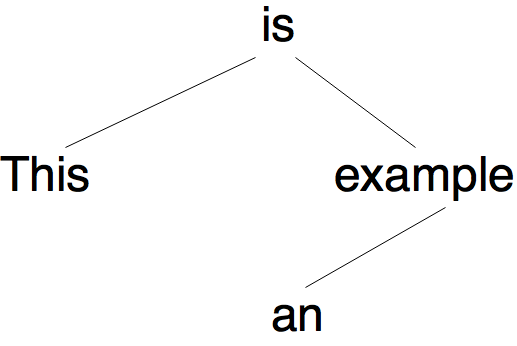
\includegraphics[scale=0.4]{DependencyTree.png}
   \caption[An example of a Dependency Tree]{A possible dependency tree for the sentence \emph{This is an example}}
   \label{dependencyTree}
\end{figure}

In the tree (figure \ref{dependencyTree}), the word \emph{This} is dependent on \emph{is} and so is linked. \emph{an} is linked to \emph{example} in a similar way, and \emph{an example} is dependent on the verb \emph{is} and so also has a link to it. 

Once dependency trees have been created for each of the sentences a similarity algorithm is used to find sentences that are similar. The common phrases between these similar sentences are then taken and form the basis of the final summary. A language generator then combines the common phrases and arranges it to create a final set of summary sentences.

An obvious disadvantage to this method is that if only common phrases are taken from the sentences, context could be lost from some of the sentences. However, on the other hand, the use of a language generator means that a more coherent, more grammatically correct summary is formed. \\

\emph{Rule based summarisation}\index{Summarisation!Rule based}

In rule based summarisation\cite{ruleBasedSummarisation}, the process is centred around a list of pre-determined categories. With each of these categories, there is a pre-determined set of questions to be answered. 

For example, with a theoretical category \emph{Product Launch} we could have the following questions:

\begin{enumerate}
	\item What is the name of the product?
	\item What company is launching it?
	\item What type of product is it?
	\item What's new about it?
	\item What price is it retailing at?
\end{enumerate}

This represents only a subset of the possible questions we could have for this category.

To perform rule based summarisation, the first step is to analyse the document and determine which category it fits best. Once that's been determined, the next stage is to analyse the text to find answers to the questions corresponding to that category. These answers are then fed in to a natural language generator that forms sentences, and thus the summary.

Results for this method of abstractive summarisation have been promising, but the method has a major disadvantage in that the list of categories and questions needs to be pre-determined. As a result, it might not be an optimal algorithm to use for the ever-changing world of news reporting. \\

\emph{Ontology based summarisation}\index{Summarisation!Ontology based}

Methods of ontology based summarisation have been developed, primarily using domain based ontology. In this method a "domain expert" defines a domain ontology for a news event. Each new document is then classified into a topic using these domain ontologies\index{Domain Ontology}. Important phrases are determined by how close they are to items in the ontology. These phrases are then passed into a natural language generator to form the final summary sentences.

A key disadvantage to this method is that a lot of the domain ontologies has to be manually determined by the "domain experts" and so can be very time consuming. As a result this may also not be particularly optimal for summarisation of news events. \\

\textbf{Semantic based summarisation} \\

\emph{Multimodal Semantic summarisation}\index{Summarisation!Multimodal Semantic}

Multimodal semantic summarisation can work on documents that contains both text and images. First, a semantic model is built to represent the document. This model is made up of different concepts that are surmised from the text. For example, the sentence \emph{Multimodal Semantic summarisation is an example of an algorithm that performs abstractive summarisation}\index{Summarisation!Abstractive} could form the concept shown in figure \ref{multimodalSummarisation}:

\begin{figure}[ht!]
  \centering
    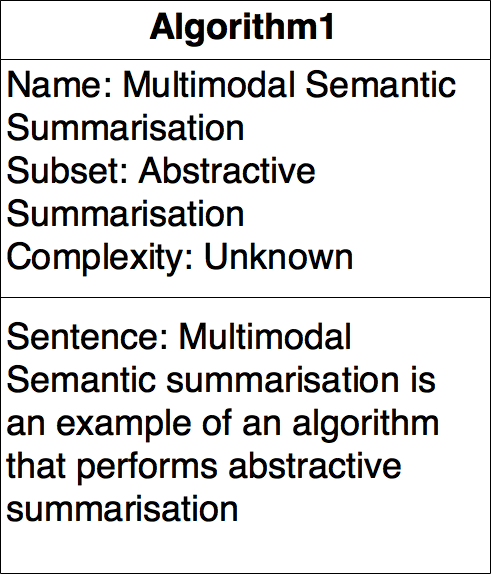
\includegraphics[scale=0.3]{MultimodalSummarisation.png}
   \caption[A concept created during multimodal semantic summarisation]{A possible concept created from the analysis of the sentence \emph{Multimodal Semantic summarisation is an example of an algorithm that performs abstractive summarisation}}
   \label{multimodalSummarisation}
\end{figure}

Concepts\index{Concept!Multimodal Summarisation} are gradually filled with more information as the entire text is analysed. Links are also added between concepts that share some relationship. For example in figure \ref{multimodalSummarisation} if there was another sentence that surmised a concept called \emph{Abstractive Summarisation} then there would be a link from \emph{Algorithm1} to that new concept. 

The next step is to rank the concepts. This is done by taking into account the completeness of the concept, and the number of links that the concept as to others. This way, the concepts are ranked by which is most important to the original document. Once the key concepts have been identified summary sentences can be generated featuring these concepts. \\

\emph{Information Item based method}\index{Summarisation!Information Item}

Information Item based summarisation\cite{informationBasedSummarisation} relies on the content of the summary being determined from an abstract representation of the original document, rather than the sentences from the document themselves. To do this, the document is first scanned so that Information Items (InIt) can be generated. An information item is defined as being "the smallest element of coherent information in a text or sentence". 

Once the information items have been created, they are then ranked using frequency analysis to find the most important predicates and entities from the original document. This step is near identical to the term frequency stage in extractive summarisation (Section \ref{extractiveSummarisation})\index{Summarisation!Extractive}. These information items that are ranked highly are then combined and fed into a natural language generator to form the final summary sentences. \\

\emph{Semantic Graph summarisation}\index{Summarisation!Semantic Graph}

Semantic Graph summarisation centres around a rich semantic graph (RSG)\index{Rich Semantic Graph}. The document is first converted into a RSG. Each node in the RSG represents a noun or verb in the document, and the links between the nodes represent the semantic and topological relations between these nouns and verbs. In the second stage, heuristic rules are used to reduce the semantic graph to a more minimalistic version. This will form the basis of the final summary. In the final step, the minimised RSG is passed into a generator that creates the final summary sentences.

The steps are outlined in the flowchart provided in figure \ref{semanticGraphSummarisation}.

\begin{figure}[ht!]
  \centering
    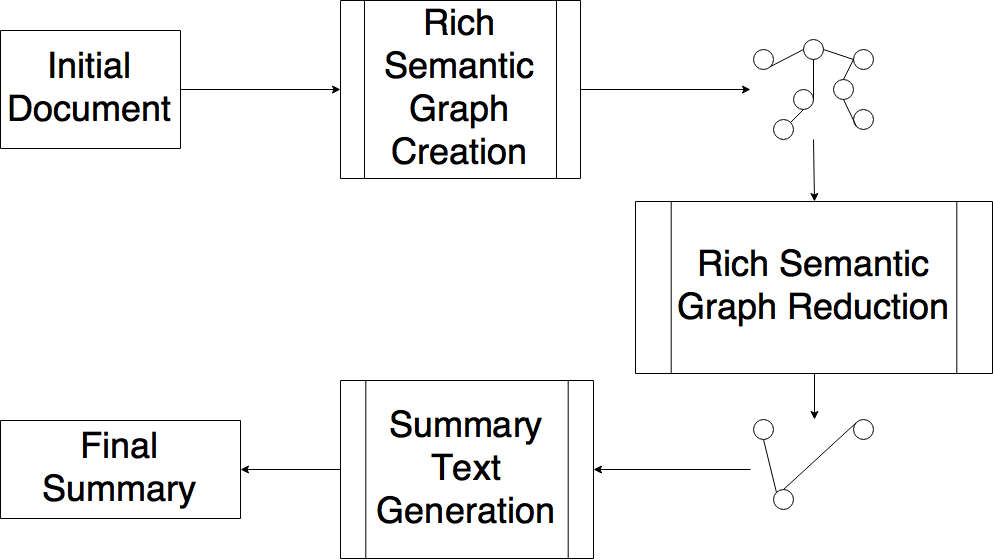
\includegraphics[scale=0.4]{SemanticGraphSummarisation.png}
   \caption[A flowchart showing the process of semantic graph summarisation]{This shows the process of semantic graph summarisation in a flowchart based on those provided in \cite{abstractiveTechniques, abstractiveTechniquesOriginal}}.
   \label{semanticGraphSummarisation}
\end{figure}

Semantic Graph summarisation has had success with producing an abstractive summary that has fewer redundant sentences, and is also good at producing grammatically correct sentences. However, it's only designed for use with a single document as input. As a result it might not be suitable as a method for summarising the multiple documents needed for the aggregator, unless it's combined with another method.

\subsection{Natural Language Processing Libraries} 

A lot of the summarisation techniques specified earlier, especially for abstractive summarisation, would require a full analysis of the semantics of a body of text. As a result, it's clear that a Natural Language Processing library will be needed for this task.

\subsubsection{Aspects of Natural Language Processing} 

\label{nlptypes}

There are several different tasks that a Natural Language Processor. A few key ones that are most likely to be required for the project are explained briefly below: \\

\begin{itemize}
	\item \textbf{Tokenisation} is the splitting of words in a given document. \\
	\item \textbf{Sentence Segmentation} is the splitting of sentences in a given document. \\
	\item \textbf{Part-of-Speech (POS) tagging} takes a list of tokens and analyses them, returning tags for each. A tag represents the grammatical function of the token in the sentence (for example if it is a noun, verb or adjective). \\
	\item \textbf{Named entity extraction} identifies the proper nouns within a document, such as people, dates or locations, as well as other categories of noun. \\
	\item \textbf{Chunking} takes a list of tags from a POS tagger and groups sets of tokens by their function in a sentence. Examples can include noun phrases and verb phrases. \\
	\item \textbf{Parsing} takes a sentence and develops a tree showing the functions of each section of the sentence. \\
	\item \textbf{Coreference Resolution} identifies noun phrases within a document that are the same. This can commonly be used for replacing pronouns with the original noun phrase. 
\end{itemize}



%%%%%%%%%%%%%%%%%%%%%%%%%%%%%%%%%%%%%%%%%%%%%%%%%%%%%%%%%%%%%%%%%%%%%%%%%%%%%%%%%%%%%%%%%%%%%%%%

\newpage

\section{Design}

\subsection{Front End Architecture\index{Front End}\index{Architecture} Diagram}

\begin{figure}[H]
  \centering
    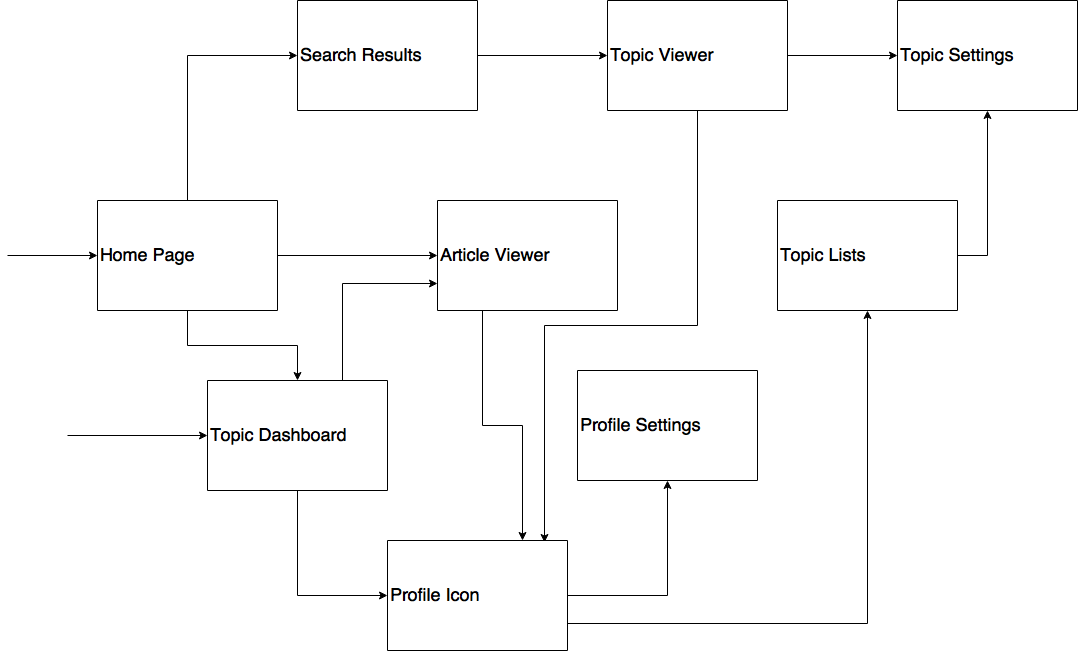
\includegraphics[scale=0.4]{FrontEndArchitecture.png}
   \caption[A basic diagram of the expected architecture of the front end]{This diagram doesn't show all anticipated connections between each facet of the application's front end. For example, the profile icon is in theory accessible anywhere when the user is logged in.}
   \label{frontEndArchitecture}
\end{figure}

\subsection{User Story}

\subsubsection{Home Page}

If a user has not logged in, the first page they will see on opening to the website will be the Home Page. The key to the design of the home page is that it's easy to get started for a user. They are presented with a large search box that they can use without having to sign in. There'll also be a row of trending articles displayed below the search bar. This row will consist of icons consisting of images and titles below, as shown in the wireframe\index{Wireframe}. There's a navigation bar at the top, that is present on all screens, with a button to register and a button to sign in on the top right, and a link to information about the application itself on the top left.

\begin{figure}[ht!]
  \centering
    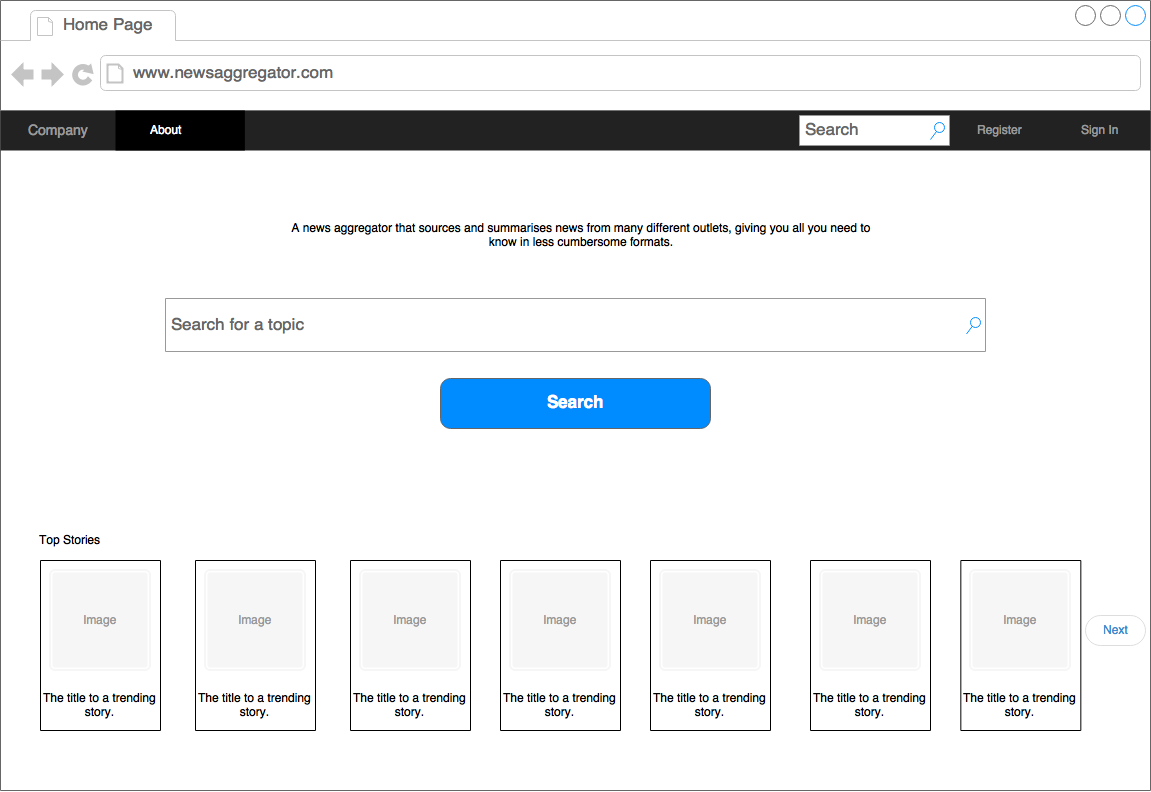
\includegraphics[scale=0.3]{HomePage.png}
   \caption[A wireframe of the Home Screen]{A key focus of the home page is that the user can easily search for articles without having to sign in or register.}
   \label{homePage}
\end{figure}

\subsubsection{Topic Dashboard}

For a user that is logged in, or alternatively a user that has logged in (or signed up) from the home page will first see the topic dashboard screen that shows sets of articles corresponding to each topic they are subscribed. For users who don't have any topics that they are subscribed to, they will instead go back to the home page. The topic dashboard initially shows leading articles from across all the topics they are subscribed to. They can drag to one direction (akin to a sideways swipe on a phone or tablet) to see articles pertaining to the next topic. 

Articles themselves are presented as panels. On a panel is an image for the article, with the title overlaid. In the top right hand corner are icons corresponding to the sources that the article has been summarised from. Leading articles (those out of the most recent that have the most sources attached) are placed in the larger panels on the top left and bottom right of the screen, as shown in the diagram.

\begin{figure}[ht!]
  \centering
    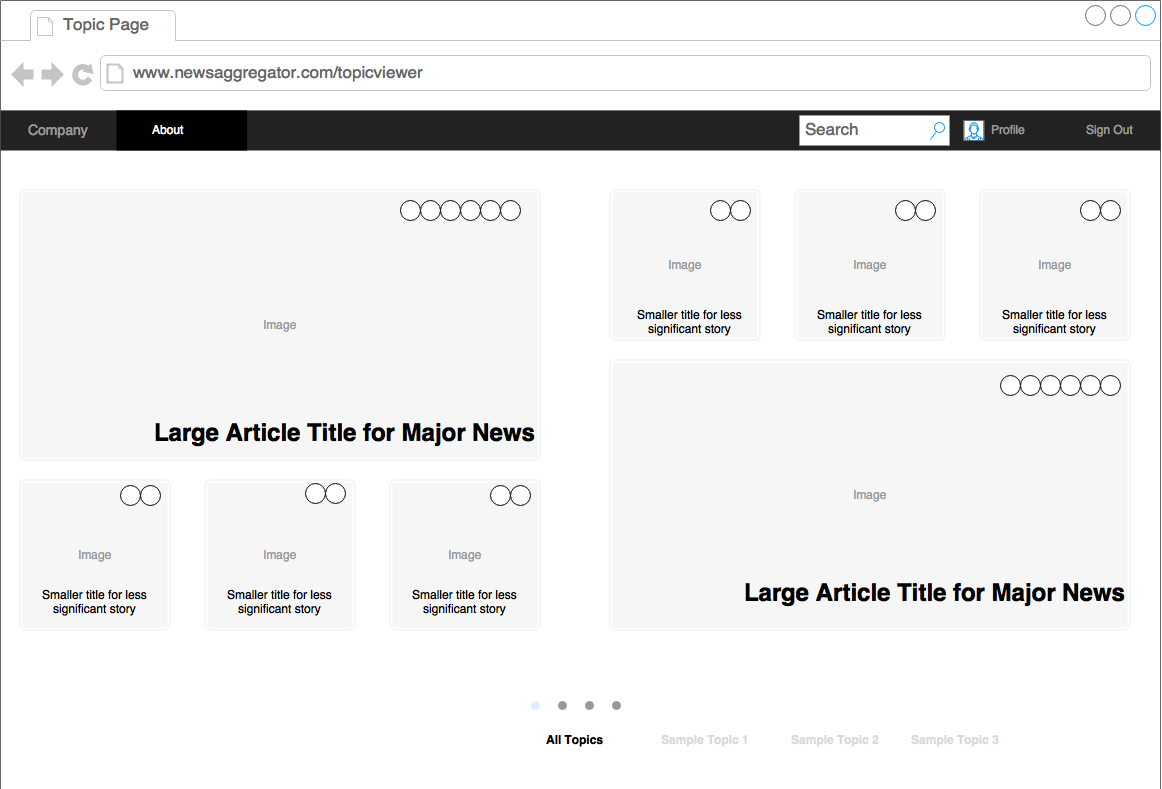
\includegraphics[scale=0.3]{TopicDashboard.png}
   \caption[A wireframe of the Topic Dashboard]{The topic dashboard has the ability to show articles across all topics, or pertaining to a specific topic.}
   \label{topicDashboard}
\end{figure}

\subsubsection{Search Results Page}

The search results page is designed to allow users to see as much as possible and do as much as possible without having to leave the page. The results are presented in the application's panel design, with an image corresponding to each panel. Below the panel, is a description of the topic, that is likely to be created from the first paragraph of the Wikipedia\cite{wikipedia}\index{wikipedia} article about that particular topic. Below this are two buttons, one to view the topic's articles, which will go to a topic viewer page (shown later), and a subscribe button. If logged in, the user is taken to the topic settings page, where they can choose any particular preferences they have for this specific topic. If the user isn't logged in, they are taken to a page allowing them to log in or register, before being taken to the preference page.

It's necessary at this stage to have a user sign in if they want to subscribe to a topic. This way, they can access their topics from anywhere. In addition to this, the search bar is still prominent on the search results page, so that users can edit their queries easily in case of minor errors.

\begin{figure}[ht!]
  \centering
    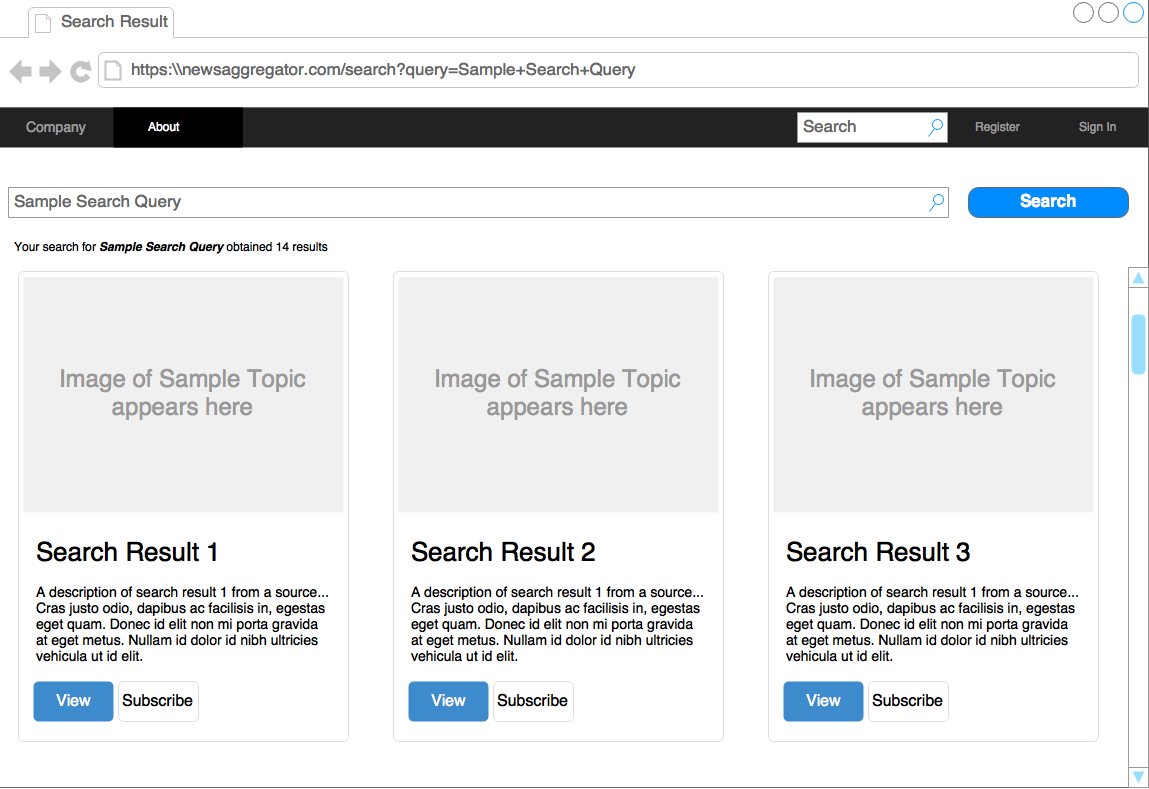
\includegraphics[scale=0.3]{SearchPage.png}
   \caption[A wireframe of the Search Results page]{The Search Results page has a focus on showing users as much information as possible about each topic.}
   \label{searchPage}
\end{figure}

\subsubsection{Topic Viewer}

The topic viewer is accessed if a user has clicked on the view button from the search results page. This screen is similar to that of the topic dashboard. Minor changes include the page control at the bottom of the screen being replaced by page statistics, including figures about how often articles are created, the number of subscribers, and the total number of hits that the page has had. The other major difference is the presence of a subscribe button in the top right hand side of the screen. As with the search results page, this leads to the topic preferences screen if logged in, and to a page prompting a user to sign in or register when not already logged in.

The remaining aspects of the screen are the same - namely the panelled articles, and the icons in the top right of each panel that indicate which sources the article originated from.

\begin{figure}[ht!]
  \centering
    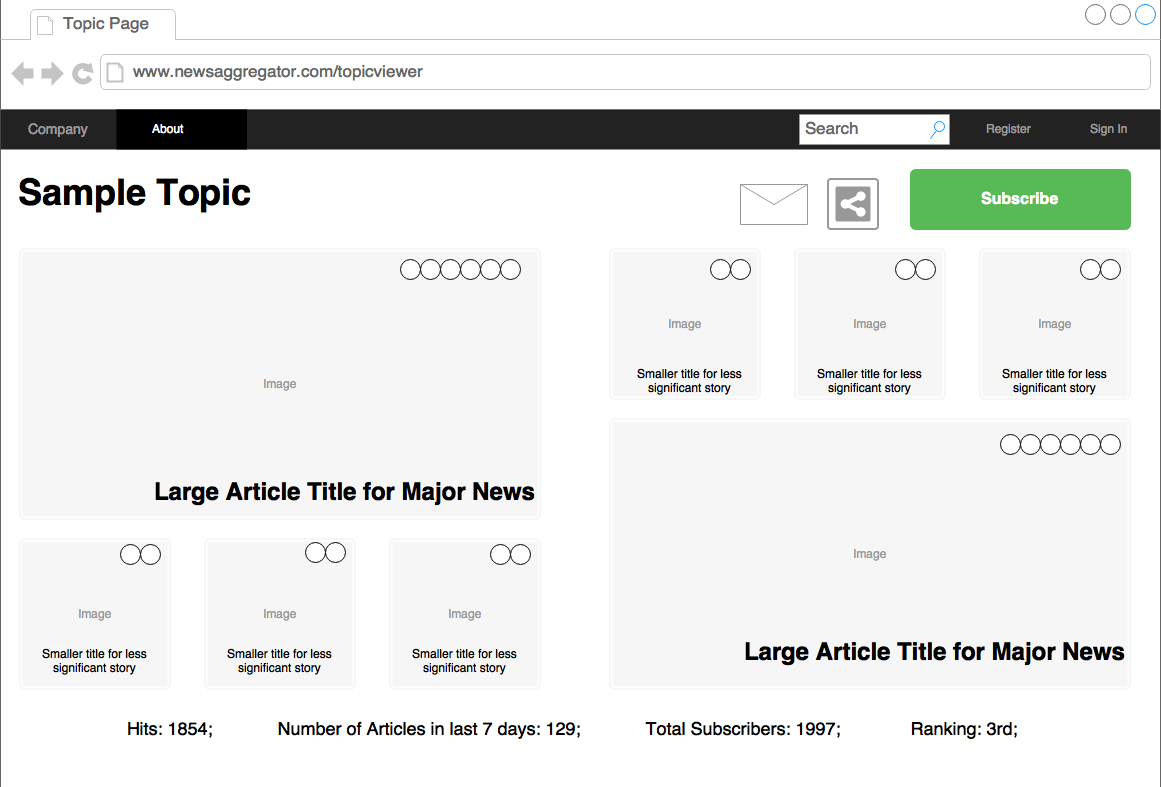
\includegraphics[scale=0.3]{TopicViewer.png}
   \caption[A wireframe of the Topic Viewer]{The topic viewer is similar in structure to the topic dashboard, but with the addition of statistics and a subscribe button.}
   \label{topicViewer}
\end{figure}

\subsubsection{Topic Settings}

The aforementioned Topic Settings page sets out two preferences from the user for a specific topic. These are namely: \\

\begin{itemize}
	\item \textbf{Should the topic's articles be included in the user's email digest?}
	
	This is answered by a simple on/off switch. \\
	
	\item \textbf{Which sources should be used to construct summaries}
	
	This aspect is done using the panelling effect used in other screens. Each news outlet's logo forms the basis of the panel, with the title of the outlet below. These panels form buttons that the user can click on to either select or deselect an outlet. The panel will either have a coloured outer rim, or an embedded effect to indicate selection. \\
\end{itemize}

\begin{figure}[ht!]
  \centering
    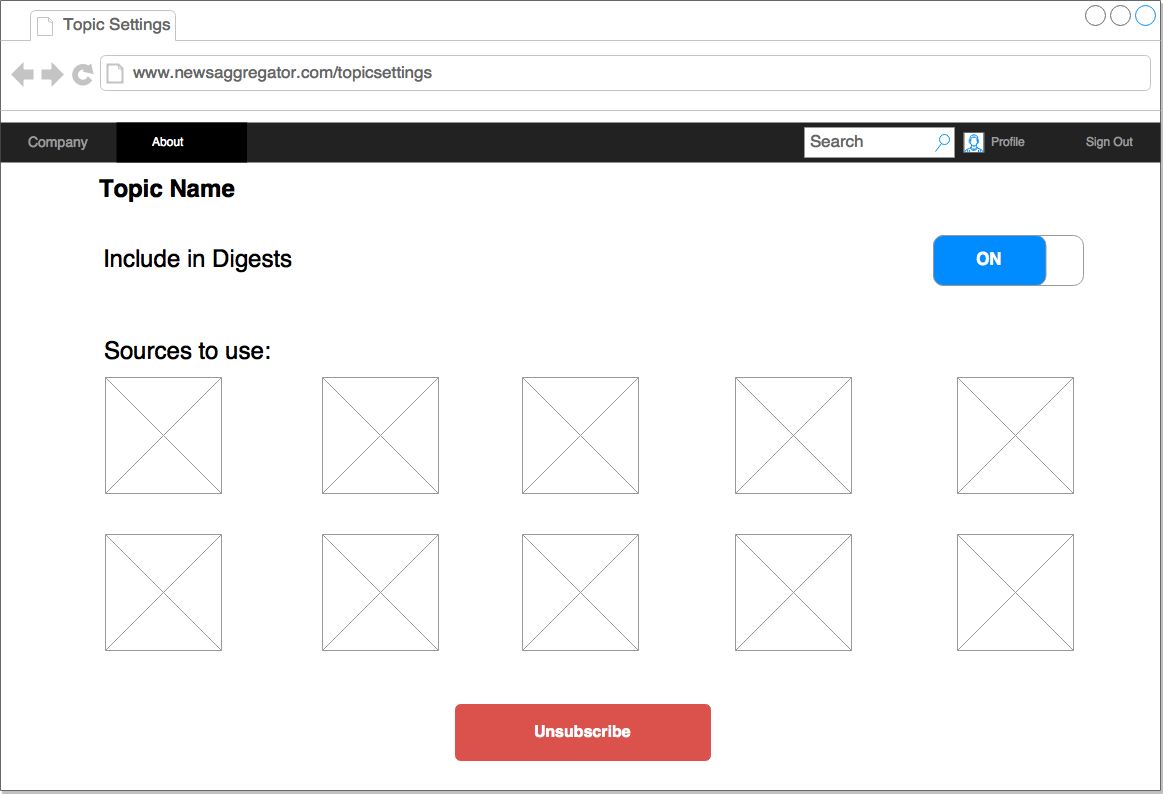
\includegraphics[scale=0.3]{TopicSettings.png}
   \caption[A wireframe of the Topic Settings page]{The Topic Settings page allows users to specify key preferences about the topic.}
   \label{topicSettings}
\end{figure}

\subsubsection{Article Viewer}

When the user clicks on an article panel in the topic viewer or topic dashboard they are presented with the summarised article itself. This screen is modelled on standard news interfaces, and produces the headline, image and article body on the left hand side of the page. On the right hand side are links to the original articles that the summary was generated from, and links to other articles that are in the same topic. 

Like most other screens in the application, there is also a share button on the top right, and an email button.

\begin{figure}[ht!]
  \centering
    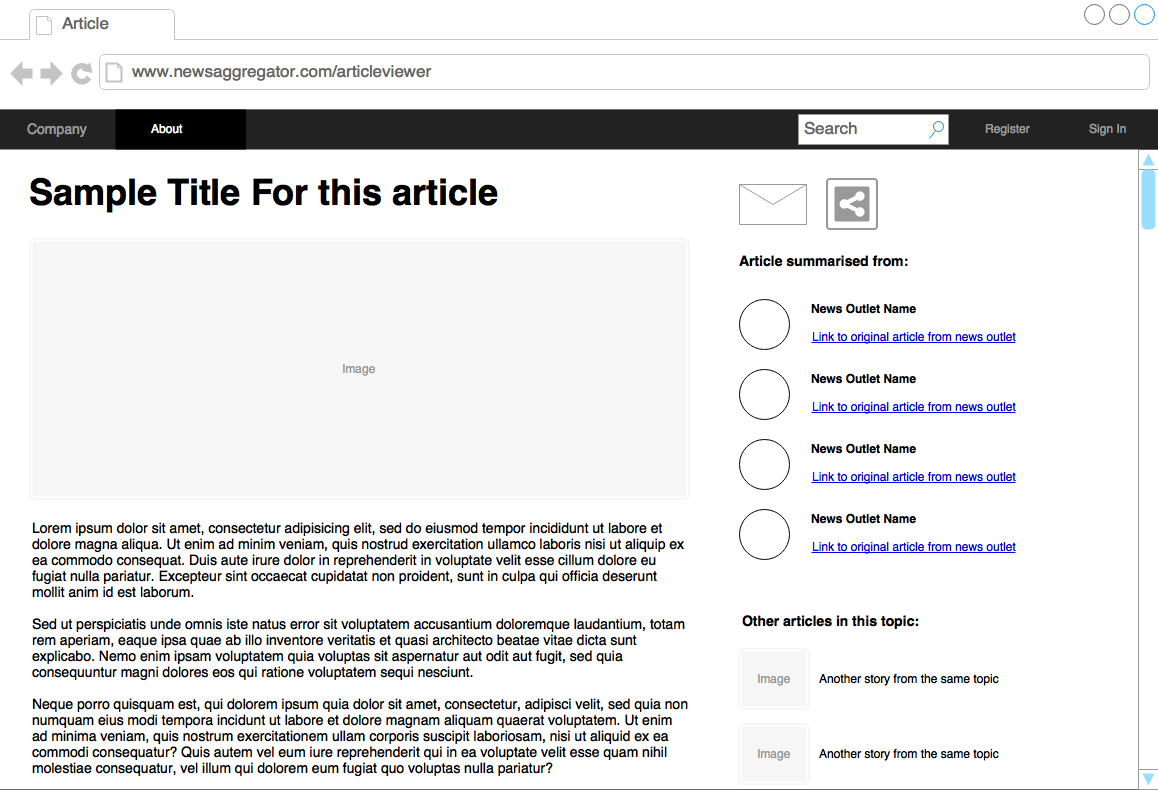
\includegraphics[scale=0.3]{ArticleViewer.png}
   \caption[A wireframe of the Article Viewer]{The Article Viewer is modelled on standard news outlets' interfaces.}
   \label{articleViewer}
\end{figure}

\subsubsection{Topic Lists}

The Topic List page is accessed by clicking on the profile button when logged in to the application. A panel appears, listing two choices - My Topics, and My Settings. This page is presented on the selection of the My Topics button.

The aim of the topic list is self-explanatory. It lists all topics that a user is subscribed to. Upon clicking on a topic in the list, a user would be taken to the Topic Settings page for that topic.

\begin{figure}[ht!]
  \centering
    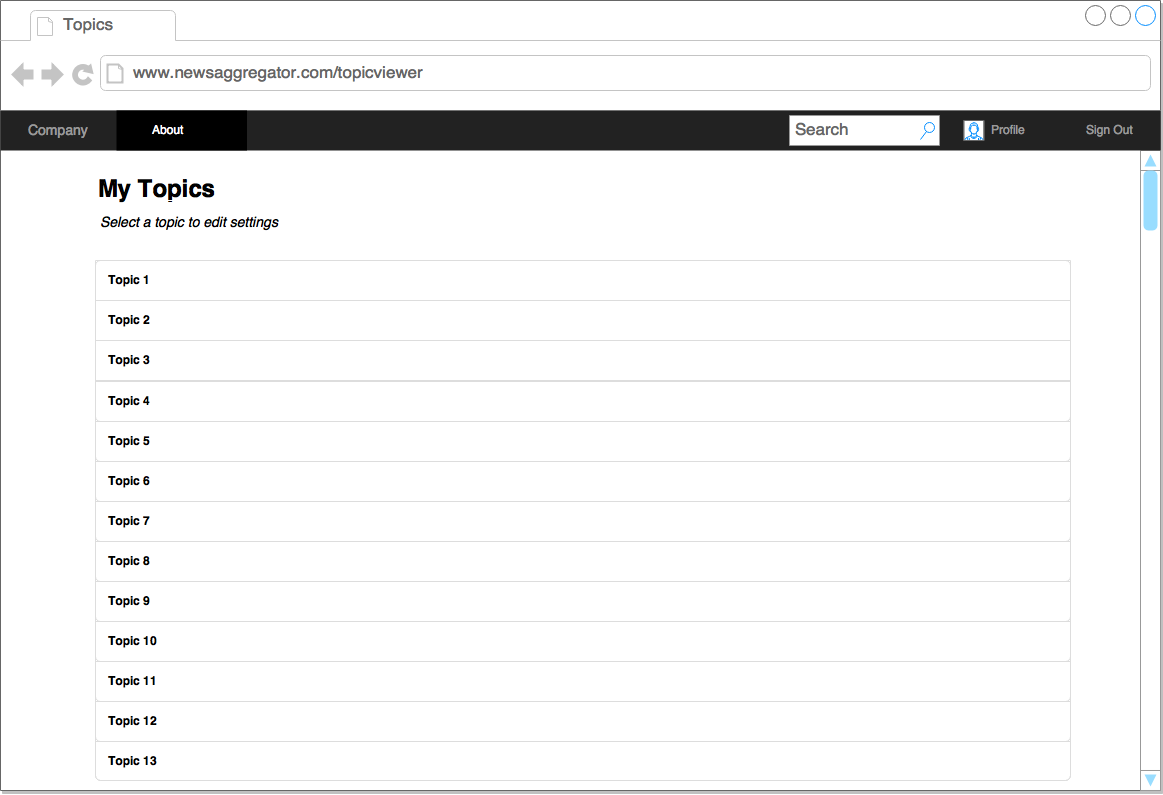
\includegraphics[scale=0.3]{UserTopics.png}
   \caption[A wireframe of the Topic List page]{The Topic List page allows users to select and adjust the settings of a topic.}
   \label{userTopics}
\end{figure} 

\subsubsection{Profile Settings}

The other option upon clicking on the profile button in the navigation bar of the application is to access the Profile Settings page. Here, the user is able to change their profile picture using the button in the top half of the page. Also present on this page are the user's digest settings. Here the user can set whether they want to receive a news digest in the morning, the afternoon, at both times, or not at all. They can also specify the email address that they wish the news digest to be sent to.

\begin{figure}[ht!]
  \centering
    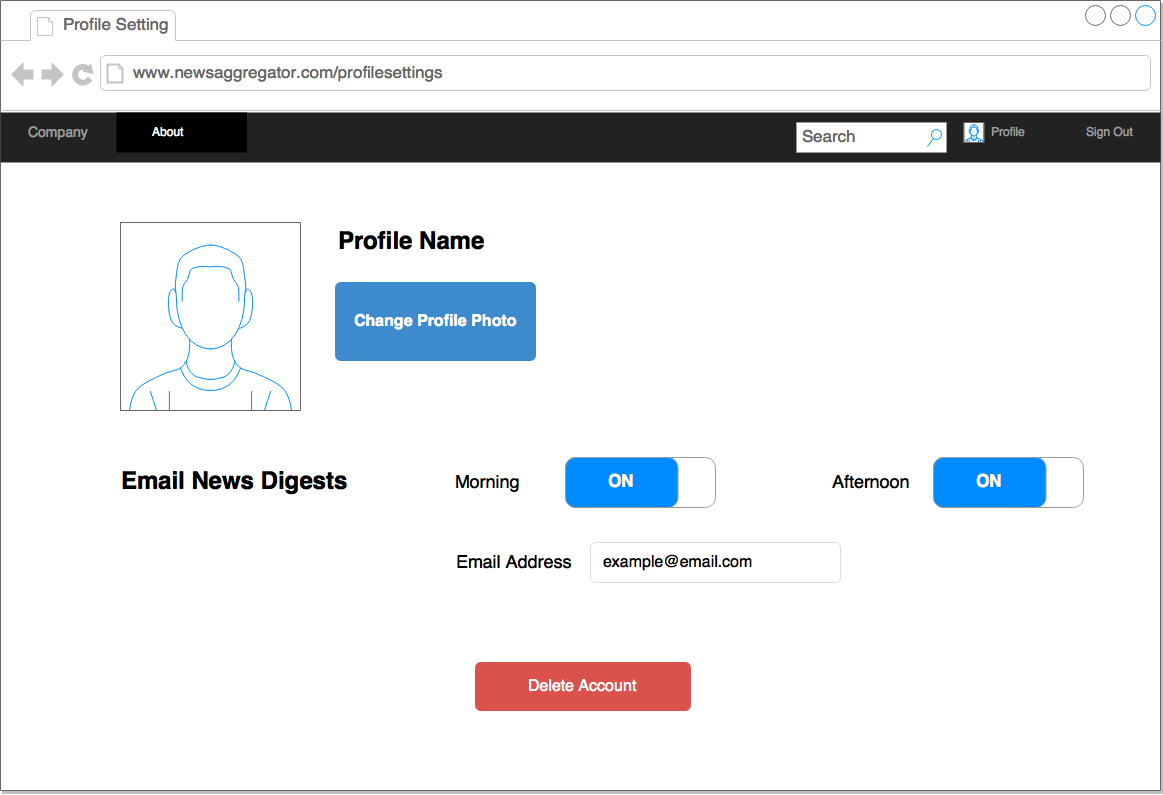
\includegraphics[scale=0.3]{ProfileSettings.png}
   \caption[A wireframe of the Profile Settings page]{The profile settings page allows the user to adjust their profile picture and digest settings.}
   \label{profileSettings}
\end{figure}

\subsection{Back End\index{Back End} Flow Diagram}

In Figure \ref{backEndArchitecture} the expected flow of the machine learning aspects of the back end is presented. The process of an article being summarised is as follows:

\begin{enumerate}
	\item The \textbf{Article Fetcher} queries the various News APIs used for new articles. \\
	\item The \textbf{Article Curator} takes the response from the News APIs and performs any scraping that may be necessary, before passing the article to the Machine Learning phases. \\
	\item The article is then passed to the \textbf{Topic Modelling}\textbf{Topic Modelling} phase, which identifies which topics it consists of. \\
	\item The \textbf{Topic Labelling}\index{Topic Labelling} section takes the results of the Topic Modelling phase, and proceeds to label its topic \\
	\item \textbf{Clustering}\index{Clustering} then occurs. The article, along with its topic label is passed to this phase, and the program pulls articles from the database that have already been assigned the same topic. These articles are then clustered, and the cluster containing this article is passed to the next phase. \\
	\item Now that the cluster has been passed, \textbf{Summarisation}\index{Summarisation} occurs on the article, which is then put in the Summarised Articles database, ready to be called for a user to read. \\
\end{enumerate}

\begin{figure}[ht!]
  \centering
    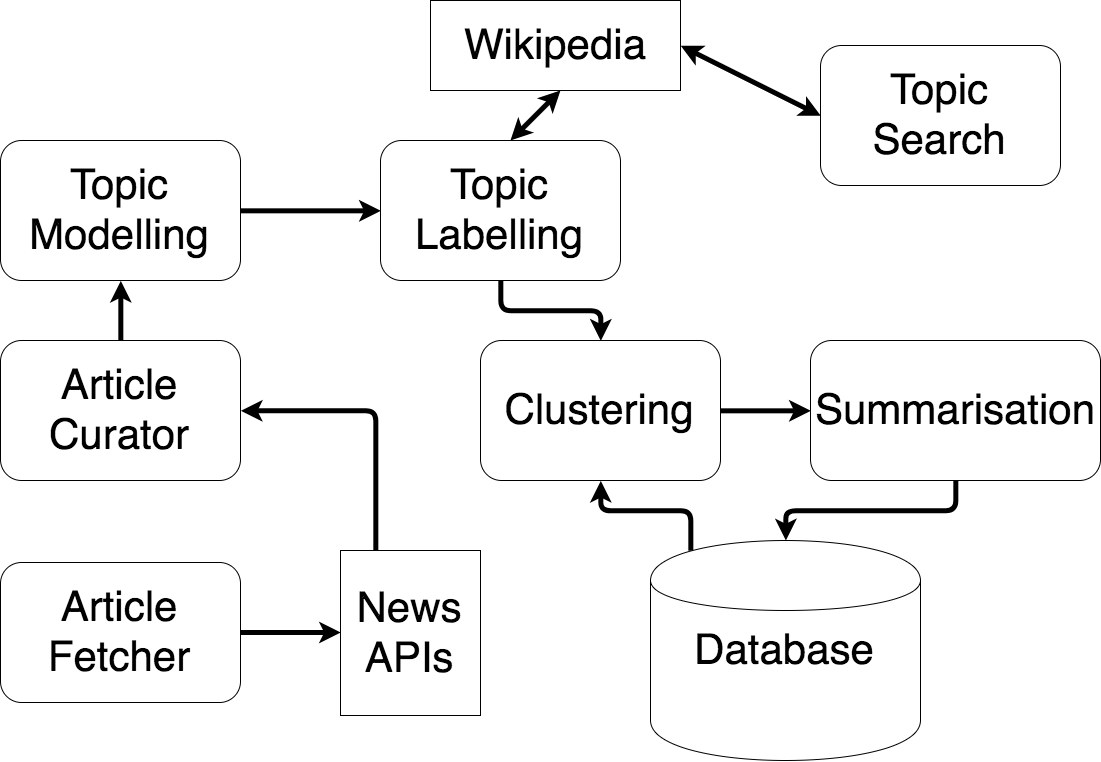
\includegraphics[scale=0.4]{BackEndArchitecture.png}
   \caption[A guide to the expected flow of the Back End]{The expected flow of the Back End.}
   \label{backEndArchitecture}
\end{figure}

\subsection{Language and Platform Choices}

\subsubsection{Front End}

The survey\index{Survey} that was conducted in Section \ref{survey} clearly presented the result that a website would be the preferred option for the application, followed by a mobile application in either iOS or Android. Therefore I've decided to follow this and create a WebApp as a primary platform. If time permits, I'll then develop the application for a second platform, which will be a mobile platform.

For the WebApp I will primarily use Bootstrap for the Interface. One design framework I used to great effect during my Industrial Placement in Summer 2016 was React and Redux\index{Redux}\index{React}. React is a JavaScript library developed by Facebook that is designed for building scalable and reusable user interfaces. Redux is a design pattern for JavaScript that is designed around a central predictable state container that is the single source of truth for a User Interface. 

The benefit of this framework is that it allows for very clean code in the user interface. This is because the concept of a single source of truth allows for data flow that is purely in only one direction, making it easier to understand.

\subsubsection{Back End}

\label{languagechoice}

The back end will be constructed using Java. The reasoning behind this is that I have experience from my Industrial Placement using Java as the basis of a server and a back end.

\subsection{Infrastructure}

\subsubsection{Hardware}

One of the first key decisions I made about the infrastructure surrounded the hardware that the server would be deployed on.

\textbf{Amazon Web Services}

Amazon Web Services (AWS) is a set of cloud computing platforms provided by Amazon. A key benefit to it is that it has a free tier, which allows for a subset of their services to be used without charge.

Some of the key platforms offered by AWS include: \\

\begin{itemize}
	\item \textbf{EC2} allows a user to create a single virtual machine for free on which to run software. This would be with a limit of 750 hours of use per month. In my case this would be used for running the back end of the News Aggregator. \\
	\item \textbf{S3} is a storage system provided by Amazon that allows a user 5GB of space for free. \\
\end{itemize} 

\textbf{Digital Ocean}

Digital Ocean is an infrastructure provider that provides "cloud computing for developers". Digital Ocean offers "droplets" that can act as virtual machines, on which I would deploy my backend. There are no free tiers, but the student pack provided by GitHub would cover the first two months of charges. 

In addition to this, one of the advantages of Digital Ocean is that if resizing of the virtual machine is necessary, it can be done in a matter of minutes, thus making the final solution very highly scalable.

In contrast though, unlike Amazon, Digital Ocean don't provide alternative microservices such as S3. Having said that, it could be argued that the droplet itself would offer that with its storage capabilities. In fact, the cheapest droplet offered by Digital Ocean (priced at \$5 a month), entails a virtual machine with a 20GB SSD disk, which is four times the amount provided by the free tier in AWS.

\subsubsection{Database}

\textbf{MongoDB}

The first database solution that I researched was MongoDB, as I have had prior experience with it. 

MongoDB is a document database that is designed to be both flexible and highly scalable. Documents are written in a format that is highly similar to JSON. This format is what results in a Mongo database being flexible, as the schema of documents in the collection can be changed quickly. 

MongoDB allows for the connection of items between tables through linking. Auto-generated "ObjectId"s (that are generated based on the timestamp) allow for easy referencing of an item in another.

A MongoDB database would have to remain in a virtual machine on either Amazon or Digital Ocean, and will therefore have to count against the storage provided by that virtual machine. \\

\textbf{DynamoDB}

DynamoDB is a No-SQL database provided by Amazon Web Services as a separate micro-service to EC2 and S3. 

The structure of a document in DynamoDB is more rigid than in MongoDB. It is primarily designed as a key-value system, with a primary key. Searching in the database is driven by this primary key, or by "secondary indexes". These secondary indexes need to be declared when the table is first created. Therefore this means that if there needs to be a schema change, the table needs to be recreated.

A DynamoDB database doesn't need to be stored in the virtual machine, but there are trade offs. Whilst Amazon Web Services provide 25GB of storage for the database as part of the free tier, there are throttles on the throughput of the database. As part of the free tier, a user is allowed to allocate 25 "units" of throughput to both reading and writing from a database, where one unit corresponds to transfer of 1KB per second. Beyond these 25 units, Amazon would start charging.

\subsubsection{Infrastructure Decisions}

\textbf{Comparison table}

Table \ref{infrastructuretable} shows the key points of comparison between the four main options for hardware and database combinations. \\

\begin{sidewaystable}
    \begin{tabular}{p{4.5cm}|p{7.75cm}|p{7.75cm}}
    \textbf{Infrastructure} & \textbf{Advantages} & \textbf{Disadvantages} \\ \hline
    AWS and MongoDB & \tabitem AWS provide free services & \tabitem Mongo would need to be hosted on the EC2 instance, or on S3, which would limit the free storage to 5GB. \\ & \tabitem Mongo provides a flexible schema, meaning that the table structure can be changed further down the line.  \\ \hline
    AWS and DynamoDB & \tabitem DynamoDB would provide 25GB of storage on its own, meaning that I wouldn't have to use the S3 storage. & \tabitem DynamoDB's key-value schema is quite rigid, meaning that there isn't much flexibility on the model.\\ & & \tabitem The throttling of reads and writes by DynamoDB could severely impact the performance of key back end tasks.\\ \hline
    Digital Ocean and DynamoDB & \tabitem Digital Ocean offers the ability to resize the server as needs be within a matter of minutes. & \tabitem As before, there are some key issues regarding the speed of DynamoDB whilst on the free tier. \\ & &\tabitem This solution would involve maintenance of a database solution provided by one company, and a server on another, which is potentially quite wasteful.  \\ \hline
    Digital Ocean and MongoDB & \tabitem MongoDB database can be stored comfortably on the Digital Ocean droplet & \tabitem Whilst covered by vouchers for the first two months of use at least, the Digital Ocean instance would require expenditure if used for longer than that period, versus AWS EC2 which would be free for at least twelve months.\\ & \tabitem The flexibility of the MongoDB model would mean that fields can be removed and added easily from the schema, allowing for further changes down the line. \\
  \end{tabular}
  \caption[Advantages and Disadvantages of different Infrastructure combinations]{Comparing the advantages and disadvantages of potential combinations of hardware and database options.}
  \label{infrastructuretable}
\end{sidewaystable}


\textbf{Decision Process}

I tried all possible combinations listed in table \ref{infrastructuretable} before finally arriving at the decision of using Digital Ocean and MongoDB.

I initially started with the configuration with AWS and MongoDB. However, it became clear quite quickly that there was a distinct possibility that the memory provided by AWS would not be sufficient to hold a large number of articles (about six weeks or greater) in the database. There certainly would not be scope for adding extra outlets near the end of the project.

In an attempt to counter this, and trying to avoid solutions that would require the spending of money, I then switched the database option to DynamoDB. This worked well for a time, but as the database grew, it became clearer that the throttling of the read and write operations to my database was going to cause major issues down the line for my background jobs on the server, as well as for simple API methods. In order to counteract this, I resolved that I would use vouchers for AWS from the GitHub student pack in order to fund some extra read-write operations per second.

Having resolved to do this, I then decided to make use of Digital Ocean. This was because I wanted to experiment to see the effects of having an instance with extra RAM would do for the running of my program, and knew that the vouchers on the GitHub student pack would easily cover a Digital Ocean droplet until the end of the project. What I found was that my background jobs (such as pulling in articles, labelling, clustering and summarisation) were being performed faster in general, and so I decided to permanently move to Digital Ocean.

In the end, a final nail in the coffin for my use of Amazon Web Services came when I wanted to change the way my articles table worked in the database. I had wanted the ability to search by date published (as I was considering at the time removing articles published before a certain date), but found that I would have to recreate my entire table in order to add this functionality to my table. As a result, and combined with the fact I now had a much larger amount of storage space on my new Digital Ocean droplet, I took the decision to make a new MongoDB database, knowing that it was still early enough in the development process that losing all my previous database work would not affect the finished product, or the development timeline.



%%%%%%%%%%%%%%%%%%%%%%%%%%%%%%%%%%%%%%%%%%%%%%%%%%%%%%%%%%%%%%%%%%%%%%%%%%%%%%%%%%%%%%%%%

\newpage

\section{Implementation}

\subsection{Database Schema}

\subsubsection{Schema Diagram}

Figure \ref{dbschema} shows the basic components of the various collections in the Mongo Database, along with some of the connections involved. Further details on each are given in each of the following sections.

\begin{figure}[ht!]
  \centering
    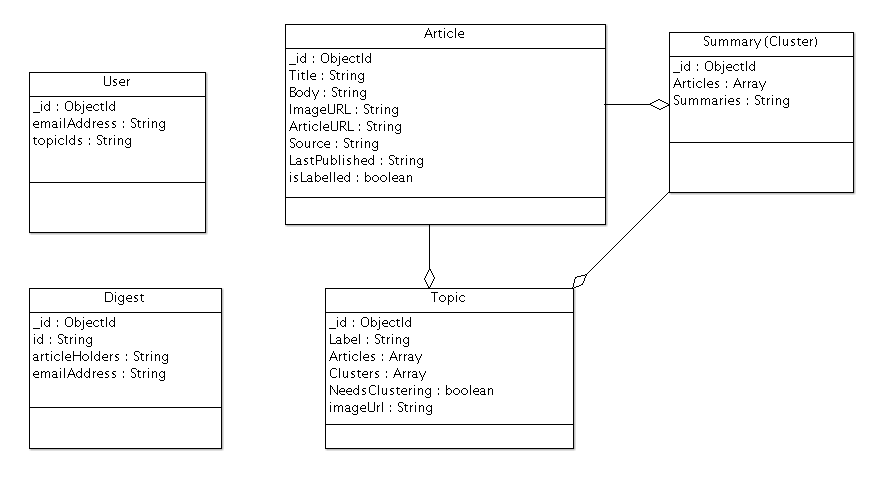
\includegraphics[scale=0.5]{dbschema.png}
   \caption[A diagram of the MongoDB schema]{A diagram of the core MongoDB schema.}
   \label{dbschema}
\end{figure} 

\subsubsection{Articles}

A sample document for an article can be seen below:

\begin{lstlisting}[language=json, firstnumber=1, caption={A sample document in the Article table}]
{
    "_id" : ObjectId("591df7cfacea820abe29709f"),
    "Title" : "Kirsten, Simons on five-man panel in hunt for new SA coach",
    "Body" : "Cricket South Africa has nominated a five-man panel including two former national coaches, Gary Kirsten and Eric Simons, to recommend a suitable candidate for the position of head coach, which it aims to fill by the beginning of September
    ...
    ",
    "ImageURL" : "http://www.espncricinfo.com/db/PICTURES/CMS/157600/157626.5.jpg",
    "ArticleURL" : "http://www.espncricinfo.com/southafrica/content/story/1098337.html",
    "Source" : "espn-cric-info",
    "LastPublished" : "2017-05-18T10:42:38Z",
    "isLabelled" : true
}
\end{lstlisting}

The purpose of the article table is for storage of raw article data that has been brought in by the article fetcher. Most fields are self explanatory. The \emph{isLabelled} field is defaulted to false when an article is first brought in, and is then changed to true when the Topic Labeller has labelled it. This is present so that articles that either weren't labelled, or caused an error when being labelled, can be found with a simple search in the database.

\subsubsection{Topics}

A sample document for a topic can be seen below:

\begin{lstlisting}[language=json, firstnumber=1, caption={A sample document in the Topics table}]
{
    "_id" : ObjectId("591df830acea820aebf55465"),
    "Label" : "Opposition (politics)",
    "Articles" : [ 
        ObjectId("591e172dacea820aebf55a74"), 
        ObjectId("5925f959acea821a75b831bc"), 
        ObjectId("59281cddacea821ab611d3ed"), 
        ObjectId("59291a47acea82594af9ef53"), 
        ObjectId("592aa5daacea8264125210d3")
    ],
    "Clusters" : [ 
        ObjectId("591f8bc7acea821e031f4dc6")
    ],
    "NeedsClustering" : true,
    "imageUrl" : "https://upload.wikimedia.org/wikipedia/commons/d/d1/Stand_in_opposition_city_hall_boston.jpg"
}
\end{lstlisting}

A topic object is a core concept in the back end. It keeps references to all articles that have been labelled with that topic, and also holds references to all the clusters (summaries) that are produced from these articles. The \emph{imageUrl} field holds either the lead image for the corresponding Wikipedia article, or a placeholder if the Wikipedia article doesn't have an image. 

The \emph{NeedsClustering} flag performs a similar function to the \emph{isLabelled} flag in the Articles table. It is defaulted to true, and is changed to false once all the clustering (but not necessarily summarisation) is completed. It is used again to find topics that may have "slipped through the cracks", either due to an error, or for some other reason. 

\subsubsection{Clusters}

A sample document for a cluster can be seen below:

\begin{lstlisting}[language=json, firstnumber=1, caption={A sample document in the Summaries table}]
{
    "_id" : ObjectId("591e47f7acea8221dcb97c42"),
    "Articles" : [ 
        ObjectId("591df7cfacea820abe2970a9"), 
        ObjectId("591df7cfacea820abe2970b2")
    ],
    "Summaries" : "{\"[daily-mail,the-guardian-uk]\":[{\"sentence\":\"President Donald Trump says he's 'very close' to naming an FBI director.\",\"sentencePosition\":0.0,\"absoluteSentencePosition\":0,\"identifier\":0,\"relatedNodes\":[],\"source\":\"daily-mail\"},{\"sentence\":\"Trump confirmed Thursday afternoon that former Democratic Sen. Joe Lieberman is a favorite for the position.\",\"sentencePosition\":0.019230769230769232,\"absoluteSentencePosition\":1,\"identifier\":1,\"relatedNodes\":[],\"source\":\"daily-mail\"},{\"sentence\":\"'We're very close to an FBI director,' Trump told reporters shouting questions at him as he met with the Colombian president in the Oval Office.\",\"sentencePosition\":0.038461538461538464,\"absoluteSentencePosition\":2,\"identifier\":2,\"relatedNodes\":[],\"source\":\"daily-mail\"},{\"sentence\":\"'Soon,' he added.\",\"sentencePosition\":0.057692307692307696,\"absoluteSentencePosition\":3,\"identifier\":3,\"relatedNodes\":[],\"source\":\"daily-mail\"}
    ...
    ]}"
}
\end{lstlisting}

An object in this table represents a Summary, and corresponds to the Clusters array in a Topic. It contains an array of references to the original articles used for the summarisation.

The \emph{Summaries} field is a string representation of a map object, with the values representing to a summary, and the corresponding key representing a combination of articles used to make that summary (represented using their sources). For example, in the full version of the sample document, there would be three keys in the string representation:

\begin{itemize}
	\item \textbf{[daily-mail,the-guardian-uk]}, for a summary using sources from \emph{The Daily Mail} and \emph{The Guardian}.
	\item \textbf{[daily-mail]}, for a summary using sources from \emph{The Daily Mail} and \emph{The Guardian}.
	\item \textbf{[the-guardian-uk]}, for a summary using sources from \emph{The Daily Mail} and \emph{The Guardian}. \\
\end{itemize}

These represent all the possible permutations (of size greater than zero) of the articles in the cluster. Its primary use is in the customisation offered to users, that can be seen in more detail in section \ref{frontendimplementation}.

\subsubsection{Users}

A sample document for a User can be seen below:

\begin{lstlisting}[language=json, firstnumber=1, caption={A sample document in the Users table}]
{
    "_id" : ObjectId("592c5288acea82147ca7f0d1"),
    "emailAddress" : "fake@gmail.com",
    "topicIds" : "[{\"topicId\":\"591e3c74acea821e2b7e6c02\",\"sources\":[\"wikipedia\",\"business-insider-uk\",\"daily-mail\",\"espn-cric-info\",\"metro\",\"mirror\",\"newsweek\",\"sky-sports-news\",\"the-telegraph\",\"the-times-of-india\",\"bbc-news\",\"bbc-sport\",\"bloomberg\",\"cnn\",\"cnbc\",\"espn\",\"four-four-two\",\"the-washington-post\",\"the-wall-street-journal\",\"associated-press\",\"the-guardian-uk\"],\"digests\":false}]"
}
\end{lstlisting}

A user object is very simple. The only field that is not necessarily self-explanatory is the \emph{topicIds} field. 

This is an array of strings, with each string forming a representation of a user's topic subscription (the topic being represented by the field marked \emph{topicId}), and the settings for that topic. The two core settings for each subscription is the digests setting (a boolean flag indicating whether a user wants to receive email digests that include this topic), and a list of sources that the user would like their news to default to (further information on this feature can be seen in section \ref{frontendimplementation}). By default, when a user subscribes to a topic, defaults is set to false, and sources is represented by a list comprising all possible sources.

\subsubsection{Digests}

A sample document for a digest can be seen below:

\begin{lstlisting}[language=json, firstnumber=1, caption={A sample document in the Digests table}]
{
    "_id" : ObjectId("591ec5c433625db581d77cc6"),
    "id" : "591ec5c433625db581d77cc6",
    "articleHolders" : "[{\"topicId\":\"593020de5826a72aa697a201\",\"articleId\":\"59322bc5acea820dd0c7ef37\",\"title\":\"Elon Musk 'intrigued' by India's objective of all-electric cars by 2030 - Times of India\",\"imageUrl\":\"http://timesofindia.indiatimes.com/photo/msid-58964385/58964385.jpg?53722\",\"lastPublished\":\"2017-06-03T08:40:00Z\"},{\"topicId\":\"5930210d5826a72aa697a227\",\"articleId\":\"59324084acea820dd0c7f65b\",\"title\":\"Kathy Griffin loses ALL of her tour gigs in wake of Trump scandal\",\"imageUrl\":\"http://i.dailymail.co.uk/i/pix/2017/06/03/05/410C672100000578-0-image-a-41_1496464334669.jpg\",\"lastPublished\":\"2017-06-03T04:39:14Z\"},{\"topicId\":\"593020de5826a72aa697a201\",\"articleId\":\"59323dddacea820dd0c7f566\",\"title\":\"Putin says hacking of Democratic Party may have been CIA false flag op\",\"imageUrl\":\"http://i.dailymail.co.uk/i/pix/2017/06/03/05/410C6AD500000578-0-image-a-92_1496463783859.jpg\",\"lastPublished\":\"2017-06-03T04:28:04Z\"}
    ...
    ",
    "emailAddress" : "specialk109@gmail.com"
}
\end{lstlisting}

A digest document represents a single daily digest for a user. Thus, a user who gets daily digests would have a single object for each day. Having said a user would have a single object for each day, it's worth pointing out that the digests are not linked to the User object. Whilst there is no concrete justification for this to be the case either way, a reason for the digests table and users table to not be linked in some way is that they simply don't need to be. A user is never called when a digest is retrieved, and similar a digest is never called when a user is retrieved.

The \emph{articleHolders} field in the document above represents the articles in a digest. It is an array of strings, with each string a JSON representation of an object containing a topic id, article id, and basic information about the cluster (title, image url, and a publishing date). The reasoning behind having the topic id in addition to the cluster is due to the pattern matching employed in the URL for the article viewer on the website (this is explained in further detail in section \ref{frontendimplementation}).

\subsection{Potentially Useful APIs}

\subsubsection{News Outlets}\index{News!Outlets}

\textbf{Readership statistics for selected outlets in the United Kingdom\index{United Kingdom}}

Statistics below are taken from the \emph{Digital News Report 2016}\cite{digitalNewsReport}\index{Digital News Report} by the Reuters Institute for the Study of Journalism\cite{reutersInstitute}\index{Reuters Institute for the Study of Journalism}. Viewership is given as a percentage of people who say they use the outlet at least weekly.

\begin{table}[H]
	\centering
	\begin{tabular}{l|c|r}
		\textbf{Outlet} & \textbf{Viewership} &\textbf{Political Stance} \\ \hline
		BBC\index{BBC} & 51\% & Neutral \\ \hline
		Mail Online\index{Mail Online} & 17\% & Right \\ \hline
		Huffington Post\index{Huffington Post} & 14\% & Left \\ \hline
		The Guardian & 14\% & Left \\ \hline
		Sky News Online\index{Sky News} & 11\% & Neutral \\ \hline
		The Telegraph Online\index{Telegraph, The} & 9\% & Right \\ \hline
		The Independent\index{Independent, The} & 6\% & Centrist \\ \hline
	\end{tabular}
	\caption[Readership statistics for selected UK outlets]{Readership statistics for selected outlets in the United Kingdom}
	\label{viewershipFigures}
\end{table}

\textbf{\\The Guardian\cite{guardian}}

\emph{The Guardian}\index{Guardian, The} is a UK newspaper that commands about 14\% of the viewership as outlined in Table \ref{viewershipFigures}. It is also known for having an API that allows a user full and free access to all articles, including the article text itself. The API can access any article dated on or after 1999, and as long as not used for a commercial purpose, is completely free to use. 

To obtain an article from \emph{The Guardian} there are two calls that need to be made. First, we make a call to the search endpoint, which returns a JSON object similar to this:

\begin{lstlisting}[language=json, firstnumber=1, caption={A sample response to an API call to The Guardian}]
{
    "response": {
        "status": "ok",
        "userTier": "free",
        "total": 1,
        "startIndex": 1,
        "pageSize": 10,
        "currentPage": 1,
        "pages": 1,
        "orderBy": "newest",
        "results": [
            {
                "id": "politics/blog/2014/feb/17/alex-salmond-speech-first-minister-scottish-independence-eu-currency-live",
                "sectionId": "politics",
                "sectionName": "Politics",
                "webPublicationDate": "2014-02-17T12:05:47Z",
                "webTitle": "Alex Salmond speech - first minister hits back over Scottish independence - live",
                "webUrl": "https://www.theguardian.com/politics/blog/2014/feb/17/alex-salmond-speech-first-minister-scottish-independence-eu-currency-live",
                "apiUrl": "https://content.guardianapis.com/politics/blog/2014/feb/17/alex-salmond-speech-first-minister-scottish-independence-eu-currency-live"
            }
        ]
    }
} 
\end{lstlisting}

From this, we extract the apiUrl, and call this, with the API key in the request headers. This will return the raw text for the article. \\

\textbf{News API}

A major issue is that most newspapers (for example, \emph{The New York Times}\cite{newYorkTimes}\index{New York Times}) only give the first paragraph to an article in their API, and don't give out their full articles as standard. There are solutions, such as Webhose\cite{webhose}\index{Webhose}, that offer feeds into this outlets, but at either a cost, or with a very limited number of requests per month. 

News API\cite{newsApi}\index{News API} is a company that provides an API to get headlines for over seventy different news outlets. A call returns data in the JSON format as follows:

\begin{lstlisting}[language=json, firstnumber=1, caption={A sample response to an API call to News API}]
{
"status": "ok",
"source": "the-next-web",
"sortBy": "latest",
"articles": [
{
	"author": "Abhimanyu Ghoshal",
	"title": "Are these ridiculous headphones the way forward for music tech?",
	"description": "All the amazing tech we now have at our disposal for enjoying music is closing us off from other people instead of bringing us together. Is there hope yet?",
	"url": "https://thenextweb.com/gear/2017/01/26/can-music-tech-make-us-sociable-again/",
	"urlToImage": "https://cdn3.tnwcdn.com/wp-content/blogs.dir/1/files/2017/01/Vinci-hed-1.jpg",
	"publishedAt": "2017-01-26T13:12:10Z"
}
]
}
\end{lstlisting}

We can use the url provided for each of these results to get to the webpage of the corresponding article. However at this stage I'll need to create a scraper to extract the raw content of the article. There could be copyright implications for this step, even though the final production summary won't look the same as the raw content. These implications will be fully examined in the final report.

News API counts amongst its 70 sources the following: \\

\begin{itemize}
	\item BBC News \index{BBC}
	\item Mail Online \index{Mail Online}
	\item \emph{The Telegraph} \index{Telegraph, The}
	\item \emph{The New York Times} \index{New York Times}
	\item Associated Press \index{Associated Press}
	\item \emph{The Independent} \index{Independent, The}
	\item \emph{The Daily Mirror} \index{Daily Mirror, The} \\
\end{itemize}

News API also has \emph{The Financial Times}\index{Financial Times, The} and \emph{The Guardian}\index{Guardian, The}, although these are left off the list above as they have their own fully accessible APIs.  

\textbf{Wikipedia}

Wikimedia\index{Wikimedia} (the parent company for Wikipedia\cite{wikipedia}) provides documentation for the Wikipedia\index{Wikipedia} API on its website MediaWiki website. Here, I can search using the search term that a user has used (perhaps in searching for a topic), and get a result that is as follows:

\begin{lstlisting}[language=json, firstnumber=1, caption={A sample response to an API call to Wikipedia's API}]
{
    "query": {
        "searchinfo": {
            "totalhits": 4152
        },
        "search": [
            {
                "ns": 0,
                "title": "Albert Einstein",
                "snippet": "&quot;<span class=\"searchmatch\">Einstein</span>&quot; redirects here. For other uses, see <span class=\"searchmatch\">Albert</span> <span class=\"searchmatch\">Einstein</span> (disambiguation) and <span class=\"searchmatch\">Einstein</span> (disambiguation). <span class=\"searchmatch\">Albert</span> <span class=\"searchmatch\">Einstein</span> (/?alb?rt ?a?n?ta?n/; German:",
                "size": 124479,
                "wordcount": 13398,
                "timestamp": "2015-05-10T12:37:14Z"
            },
            ...
}
\end{lstlisting}

The search query can be altered to provide different information, such as the URL for the lead image, which can be used to show previews of various items to users. The Wikipedia API can also be used in the topic labelling aspect of the Machine Learning techniques (see Section \ref{TopicLabelingTechniques}).

\subsection{Potentially useful libraries}

\subsubsection{Mallet}

\label{mallet}

Mallet (Machine Learning for Language Toolkit) is a java library that provides an interface for various natural language-based machine learning tasks. These tasks include:

\begin{itemize}
	\item Document Classification
	\item Sequence Tagging
	\item Clustering
	\item Topic Modeling
	\item Information Extraction \\
\end{itemize}

\textbf{Mallet in Topic Modeling}

Mallet is particularly useful for Topic Modeling. Mallet uses a corpus in the form of a list of strings in order to train a set of topics. The library trains the topics using Gibbs Sampling and Latent Dirichlet Allocation.

Mallet also provides an inferencer that allows a user to submit a new document and receive a list of probabilities. Each of these probabilities shows the likelihood that the corresponding topic is an accurate classification of the document we are testing. Thus the user can then infer the actual topics that the document is about by simply taking the topics with the highest probabilities. 
 

\subsubsection{Natural Language Processing}

There are several Natural Language Processing libraries available. The following are designed for use in Java: \\

\textbf{Apache OpenNLP} \\

OpenNLP is an open source library developed by Apache. The aim of the project is to support the basic aspects of natural language processing.

OpenNLP supports all of the basic tasks that were specified in section \ref{nlptypes} with varying degrees of success, plus "document categorisation".

Document Categorisation, as the name suggests, takes a document and categorises it. This could potentially be used in the topic modelling phase, but has the disadvantage that it doesn't come with a model for training, and the user of the library has to create their own. This is a contrast to the Mallet library, which can create a model when the user passes in the raw data.

When it comes to the other key tasks of Natural Language Processing, OpenNLP provides flexibility on models. They provide a default model in a variety of languages, including English. However, there is at least one different model file for each task, so space constraints need to be considered. \\

\emph{Name Finder}

For using the name finder, there are different model files, depending on what types of proper nouns a user is looking for. These are: 

\begin{itemize}
	\item Date
	\item Location
	\item Money
	\item Organisation
	\item Percentage
	\item Person
	\item Time \\
\end{itemize} 

\emph{Space Constraint Table}

Table \ref{opennlpspace} shows each model and their respective sizes. As Apache's recommended method to bring the files in to the program is through the Java class FileInputStream their sizes can be important, as they make use of the Java heap.

\begin{table}[H]
	\centering
	\begin{tabular}{l|l|r}
		\textbf{Model Name} & \textbf{Task} & \textbf{Size (MB)} \\ \hline
		en-chunker & Chunking & 2.6 \\ \hline
		en-ner-date & Name Finder: Dates & 5.0 \\ \hline
		en-ner-location & Name Finder: Locations & 5.1 \\ \hline
		en-ner-money & Name Finder: Money & 4.8 \\ \hline
		en-ner-organization & Name Finder: Organisations & 5.3 \\ \hline
		en-ner-percentage & Name Finder: Percentages & 4.7 \\ \hline
		en-ner-person & Name Finder: People & 5.2 \\ \hline
		en-ner-time & Name Finder: Time & 4.7 \\ \hline
		en-pos-maxent & POS Tagging & 5.7 \\ \hline
		en-sent & Sentence Detection & 0.01 \\ \hline
		en-token & Tokenisation & 0.44 \\ \hline
		\textbf{Total if all used} & & \textbf{43.55} \\ \hline
	\end{tabular}
	\caption[Space used for OpenNLP models]{A table showing the space required for the various models provided for use with OpenNLP}
	\label{opennlpspace}
\end{table}

\textbf{Stanford CoreNLP}

The Stanford CoreNLP is a toolkit provided for Java by the Stanford Natural Language Processing Group. Like Apache OpenNLP, CoreNLP also offers the same functionalities that were discussed in section \ref{nlptypes}. However, Stanford go above and beyond this list in what they can provide. Their coreference and name recognition solutions are "competition winning", whilst they also provide functionality for semantic analysis of text.

As a result, CoreNLP could have a major benefit for abstractive summarisation, through its coreference resolution. \\

\emph{Extracting elements from a document}

The following is a code snippet, taken from the Stanford CoreNLP documentation that demonstrates how to perform certain Natural Language tasks from a given annotated document. \\

\begin{lstlisting}[style=MyJava, firstnumber=1, caption={Analysing an annotated document using Stanford's CoreNLP}]

// these are all the sentences in this document
// a CoreMap is essentially a Map that uses class objects as keys and has values with custom types
List<CoreMap> sentences = document.get(SentencesAnnotation.class);

for(CoreMap sentence: sentences) {
  // traversing the words in the current sentence
  // a CoreLabel is a CoreMap with additional token-specific methods
  for (CoreLabel token: sentence.get(TokensAnnotation.class)) {
    // this is the text of the token
    String word = token.get(TextAnnotation.class);
    // this is the POS tag of the token
    String pos = token.get(PartOfSpeechAnnotation.class);
    // this is the NER label of the token
    String ne = token.get(NamedEntityTagAnnotation.class);
  }

  // this is the parse tree of the current sentence
  Tree tree = sentence.get(TreeAnnotation.class);
}

// This is the coreference link graph
// Each chain stores a set of mentions that link to each other,
// along with a method for getting the most representative mention
// Both sentence and token offsets start at 1!
Map<Integer, CorefChain> graph = 
  document.get(CorefChainAnnotation.class); 
 
\end{lstlisting}

\textbf{\\ WordNet}

WordNet is a large scale database developed by Princeton that offers a lexical database of the English language. It can primarily be used as a thesaurus, and could therefore be useful in the natural language generation of abstractive summarisation, as well as in finding similarities between sentences.

\subsection{Machine Learning}

\subsubsection{Topic Modelling}

For the Topic Modelling task I used the Mallet library, which is described in full detail in section \ref{mallet}.

There are two sections to the topic modelling phase: Training, and Estimating. \\

\textbf{Training}

For training the model, I used the ParallelTopicModel class provided by the Mallet library. The class provides a parallel implementation of Latent Dirichlet Allocation. There are several key parameters that need to be passed in to the model before it can be estimated:

\begin{itemize}
	\item \textbf{numTopics}, the number of topics to model the corpus into.\\
	\item \textbf{alphaSum} is distributed evenly across all topics. For example, an alphaSum of 1 over 100 topics would result in each topic having an alpha score of 0.01. An alpha score is viewed as a smoothing term. It ensures that the probability of a given topic being in a document is never zero.\\
	\item \textbf{beta} is similar to alpha, and is the corresponding smoothing factor ensuring that the probability of a word being in a given topic is never zero.\\
	\item \textbf{numIterations} is the number of iterations the trainer should run through before presenting a final model.\\
\end{itemize}

Initially I attempted to model topics by feeding in articles and seeing what topics came up. However, it was clear that this wasn't ideal, as frequently occurring words, such as "a", "the" and "and" were too prominent in the list of words in each topic, and thus were skewing any results from the estimation stage.

I then tried to use the provided "stoplists" file. With this file, Mallet aims to filter out common words with no real significance out of the given texts, before training topics. It became noticeable quickly though that the stoplists file wasn't extensive enough, as it was missing contracted words, such as "it's". Given the frequency of these words, I dismissed this idea and set about a new solution.

As a final solution, I decided to remove all insignificant words by removing all non-nouns from the article bodies. I did this using the Apache OpenNLP library, and found that this made (to the naked eye) the topic models look a lot better. 

My final parameters can be seen in table \ref{topicmodellingtraining}.

\begin{table}[H]
	\centering
	\begin{tabular}{l|r}
		\textbf{Parameter} & \textbf{Final Value} \\ \hline
		alphaSum & 1.0 \\ \hline
		beta & 0.01 \\ \hline
		numTopics & 500 \\ \hline
		numIterations & 1500 \\ \hline
	\end{tabular}
	\caption[Parameters for training topic models]{A table showing the final parameters chosen for the topic modelling training}
	\label{topicmodellingtraining}
\end{table}

Initially, the articles would be used to retrain the model each time a set of articles were about to be labelled. However, in the optimisation phase of the project, I changed this so that the training would happen once a week, and a model saved on file. Full details and justification can be found in section \ref{topicmodellingoptimisation}. \\

\textbf{Estimation}

The body of the article to be estimated is passed in to the model. This was initially the whole article, but after I decided to keep only nouns for training, I did the same for estimation. 

There are three key parameters for estimation. These are:

\begin{itemize}
	\item \textbf{numIterations}, which is the number of times to iterate through the model before producing a final estimate. \\
	\item \textbf{thinning}, which is the number of iterations to run before saving an interim model.\\
	\item \textbf{burn-in} is the number of iterations to perform before beginning the estimation. The reasoning behind this is that since the first iteration begins with a random distribution, the first set of iterations are unlikely to be truly representative of the actual model. The burn-in period could potentially be compared to the warm-up of an athlete. \\
\end{itemize}

After the topic model for the new article has been estimated, I prepare the result for topic labelling. To do this, I parse the data into a new custom class I created, that stores the word and the "distribution". The distribution is calculated by the Mallet library, and is an indication of the likelihood that an article belongs to a certain topic.

The final parameters chosen can be seen in table \ref{topicmodellingestimation}.

\begin{table}[H]
	\centering
	\begin{tabular}{l|r}
		\textbf{Parameter} & \textbf{Final Value} \\ \hline
		numIterations & 2500 \\ \hline
		thinning & 40 \\ \hline
		burn-in & 50 \\ \hline
	\end{tabular}
	\caption[Parameters for estimating topic models]{A table showing the final parameters chosen for the topic modelling estimation}
	\label{topicmodellingestimation}
\end{table}

\subsubsection{Topic Labelling}

When I first implemented the Topic Labelling phase of the backend, I aimed to emulate the algorithm of Lau, Grieser, Newman and Baldwin as closely as possible. This algorithm is detailed in section \ref{labellingalgorithm}. However, once this algorithm had been implemented, it was clear that there were some potential flaws when it applied to my project.

A key issue in the topic labelling phase was that of speed. The algorithm required dozens (and potentially hundreds) of calls to the Wikipedia API. There are ten calls in step two (searching Wikipedia for the original top ten topic terms), followed by calls on every single noun chunk found in step three of the algorithm. Calculating the Related Article Conceptual Overlap scores (RACO, see section \ref{RACOcalculation} would also require every single "outlink" to be found, and every category of it. Given this needs to be done for every single noun chunk found earlier, it was easy to see why this could become prohibitively costly in terms of speed. 

A simple test run using five articles from \emph{The Guardian} of varying lengths resulted in each taking at least fifteen minutes to complete the topic labelling process. Given the potential volume of articles expected per day, I reluctantly dismissed the algorithm as too expensive for the project.

In order to streamline the labelling process I removed major aspects of the algorithm. This included removing the creation of noun chunks, and the RACO calculation. I also looked to some simple heuristics, such as isolating names using the OpenNLP library and automatically adding them as labels. \\

\textbf{Brief overview of final labelling algorithm} \\

\begin{enumerate}
	\item \textbf{Find all proper names} in the article body using the Apache OpenNLP library. I used the models for Locations, Organisations and People in this phase. \\
	\item \textbf{Search Wikipedia} for the top fifteen results for each of the ten topic words provided by the modelling algorithm. \\
	\item \textbf{Retrieve text from Wikipedia articles} for all results in step two that aren't in the list of names found in step one. \\
	\item \textbf{Perform Candidate Ranking.} This step is described in more detail below. \\
	\item \textbf{Add top 18 results to candidates from step one.} The number 18 was found via trial and error, with the aim of striking a balance between too many potential labels and too few. Too many could result in a very slow clustering process, as there are too many topics that need clustering, causing a backlog. Too few could reduce accuracy. \\
\end{enumerate}

This significantly increased the speed of the algorithm, and articles that were taking fifteen minutes or more on the previous algorithm were now taking less than a minute, which I decided would be fast enough for the expected volume of articles.

A full analysis of the speed of the new topic labelling algorithm, and its role in the bigger picture of the summarisation process is outlined in the evaluation section. \\

\textbf{Brief overview of candidate ranking algorithm} \\

\begin{enumerate}
	\item \textbf{Isolate the nouns from the Wikipedia articles of every label}\\
	\item \textbf{Use nouns from step one as a corpus in a TF-IDF model} \\
	\item \textbf{Isolate the nouns from the original article} \\
	\item \textbf{For each label:}
		\begin{itemize}
			\item Calculate the sum of performing TF-IDF on each individual noun from the label's article. The TF-IDF algorithm is explained in full detail in section \ref{ClusteringTechniques}. \\
			\item Find the total number of nouns that are present in the original article that are also present in the candidate article. This is known as the crossover. \\
			\item Normalise the crossover by dividing it by the total number of nouns in the candidate article and the original article. \\
			\item Multiply the crossover by the sum of TF-IDF operations found earlier to give a final total. \\
		\end{itemize}
	\item \textbf{Order the candidates by score}, highest to lowest.\\
\end{enumerate}

\subsubsection{Clustering}

\subsection{Summarisation}

\subsubsection{Extractive Summarisation}

\subsubsection{An attempt at Abstractive Summarisation}

\subsection{Restlet}

\subsection{Server Tasks}

\subsection{Front End}

\label{frontendimplementation}

\subsection{Key Classes}

% Mention classes such as the LabelHolder and ClusterHolder here?

%%%%%%%%%%%%%%%%%%%%%%%%%%%%%%%%%%%%%%%%%%%%%%%%%%%%%%%%%%%%%%%%%%%%%%%%%%%%%%%%%%%%%%%%%

\newpage

\section{Optimisation}

\subsection{Speed Optimisations}

\subsubsection{Topic Modelling}

\label{topicmodellingoptimisation}

\subsubsection{Topic Labelling}

\subsubsection{Clustering}

\subsection{Memory Optimisations}

%%%%%%%%%%%%%%%%%%%%%%%%%%%%%%%%%%%%%%%%%%%%%%%%%%%%%%%%%%%%%%%%%%%%%%%%%%%%%%%%%%%%%%%%%

\newpage

\section{Evaluation}

\subsection{Machine Learning and Summarisation}

%Summary Evaluation Resource

\subsection{Summary Analysis}

\subsection{User Interface Evaluation}

%%%%%%%%%%%%%%%%%%%%%%%%%%%%%%%%%%%%%%%%%%%%%%%%%%%%%%%%%%%%%%%%%%%%%%%%%%%%%%%%%%%%%%%%%

\newpage

\section{Conclusion}

%%%%%%%%%%%%%%%%%%%%%%%%%%%%%%%%%%%%%%%%%%%%%%%%%%%%%%%%%%%%%%%%%%%%%%%%%%%%%%%%%%%%%%%%%

\newpage

\section{Future Work}

\subsection{Foreign Languages}

\subsection{Further Optimisations}

\subsection{Other Apps}

%%%%%%%%%%%%%%%%%%%%%%%%%%%%%%%%%%%%%%%%%%%%%%%%%%%%%%%%%%%%%%%%%%%%%%%%%%%%%%%%%%%%%%%%%

\newpage

\printbibliography[heading=bibintoc]

%%%%%%%%%%%%%%%%%%%%%%%%%%%%%%%%%%%%%%%%%%%%%%%%%%%%%%%%%%%%%%%%%%%%%%%%%%%%%%%%%%%%%%%%%

\newpage

\begin{appendices}

%%%%%%%%%%%%%%%%%%%%%%%%%%%%%%%%%%%%%%%%%%%%%%%%%%%%%%%%%%%%%%%%%%%%%%%%%%%%%%%%%%%%%%%%%

\section{Source Code}

%%%%%%%%%%%%%%%%%%%%%%%%%%%%%%%%%%%%%%%%%%%%%%%%%%%%%%%%%%%%%%%%%%%%%%%%%%%%%%%%%%%%%%%%%

\newpage

\section{API}

%%%%%%%%%%%%%%%%%%%%%%%%%%%%%%%%%%%%%%%%%%%%%%%%%%%%%%%%%%%%%%%%%%%%%%%%%%%%%%%%%%%%%%%%%

\newpage

\section{User Guide}

\end{appendices}

%%%%%%%%%%%%%%%%%%%%%%%%%%%%%%%%%%%%%%%%%%%%%%%%%%%%%%%%%%%%%%%%%%%%%%%%%%%%%%%%%%%%%%%%%

\newpage
\printindex

\end{document}